\documentclass[10pt]{beamer}
%\documentclass{article}
%\usepackage{beamerarticle}
\usepackage[style=verbose,backend=biber]{biblatex}
\usepackage{amsmath}
\usepackage{amssymb}
\usepackage{bookmark}
\usepackage{hyperref}
\newcommand{\g}{\nabla}
\newcommand{\xbold}{\mathbf{x}}
\newcommand{\citecomma}{\({}^{{}_{,}}\)}
\usetheme{CambridgeUS}
\addbibresource{main.bib}
\renewcommand{\footnotesize}{\tiny}

\title[Analysis of AG Methods]{An Empirical Analysis of the Benefits of Adaptive Gradient Methods}
\subtitle{Project done as a part of \\
CS6230 - Optimization Methods in Machine Learning}

\author{Vishwak Srinivasan \and Ayushi Patel}

\begin{document}
\begin{frame}
\titlepage
\end{frame}

\section{Introduction}
\subsection{Gradient Descent}
\begin{frame}{Gradient Descent}
\begin{itemize}
\item<1->{Gradient Descent (GD) - based methods have been a staple approach used for optimization
          in both convex and non-convex problems for many years now.
          \begin{itemize}
          \item<2->{Huge success attributed to the simplicity of the method}
          \end{itemize}
         }
\item<3->{Start with a random initialization, and follow the direction of descent.
          \begin{itemize}
          \item<4->{Direction of descent given by the negative of the gradient of a particular point.}
          \end{itemize}
         }
\uncover<5->{\[\xbold := \xbold - \eta \g f(\xbold)\]}
\end{itemize}
\end{frame}

\subsection{Modifications to Gradient Descent}
\begin{frame}{Modifications to Gradient Descent}
\begin{itemize}
\item<1->{Polyak\footfullcite{polyak} and Nesterov\footfullcite{nag} have proposed methods which \textit{provide an acceleration} to the updates.
          \begin{itemize}
          \item<2->{Collectively called \textbf{momentum based methods}}
          \end{itemize}
         }
\item<3->{Gradient descent is used as \textit{mini-batch gradient descent} in practice, which leads
          to \textit{variance in the calculated mini-batch gradients}. Methods like SVRG\footfullcite{svrg}, SAG\footfullcite{sag} and % add citations
          SDCA\footfullcite{sdca} have been proposed to help solve this problem.
          \begin{itemize}
          \item<4->{Collectively called \textbf{variance reduction methods}}
          \end{itemize}
         }
\item<5->{Choice of learning rate is cumbersome process in gradient based methods. Methods like Adam,
          Adagrad, Adadelta, RMSprop and so on \textit{adapt the learning rate} through the updates. % add citations
          \begin{itemize}
          \item<6->{Collectively called \textbf{adaptive gradient methods}}
          \end{itemize}
         }
\end{itemize}
\end{frame}

\section{Adaptive Gradient Methods}
\subsection{Introduction}
\begin{frame}{Introduction to Adaptive Gradient Methods}
\uncover<1->{General form of any adaptive gradient method is: \[\xbold_{t+1} := \xbold - \eta_{t}\g_{\xbold_{t}} f(\xbold_{t})\] where \(\xbold_{t}\) is the value of \(\xbold\) at iteration \(t\)}
\(\newline\)

\uncover<2->{Key idea of any adaptive gradient method is to \textit{modify the learning rate} based on previous updates. Following slides will discuss some ``well-known'' adaptive gradient methods used in practice briefly.}
\end{frame}

\subsection{Adagrad}
\begin{frame}{Adagrad\footfullcite{adagrad}} % add citations
\uncover<1->{Define: \[G_{t} \triangleq \mathrm{diag}\left(\displaystyle \sum_{i=0}^{t} \g f(\xbold_{i}) \odot \g f(\xbold_{i})\right)\]}
\uncover<2->{Adagrad updates parameters based on the rule below:
\begin{equation}
\label{adagrad}
\xbold_{t+1} = \xbold_{t} - \frac{\eta}{\sqrt{G_{t} + \epsilon}} \odot \g f(\xbold_{t})
\end{equation}
where \(\epsilon\) is a small value to prevent divide by zero errors
}
\end{frame}

\subsection{Adadelta}
\begin{frame}{Adadelta\footfullcite{adadelta}} % add citations
\uncover<1->{Define: \[g_{t} \triangleq \g f(\xbold_{t}) \odot \g f(\xbold_{t})\]
\[\mathbb{E}[g]_{t} \triangleq \rho\mathbb{E}[g]_{t-1} + (1 - \rho)g_{t}\]
\[\Delta \xbold_{t} \triangleq -\eta\displaystyle\frac{\sqrt{\mathbb{E}[\Delta \xbold]_{t-1} + \epsilon}}{\sqrt{\mathbb{E}[g]_{t} + \epsilon}}\odot\g f(\xbold_{t})\]
\[\mathbb{E}[\Delta \xbold]_{t} \triangleq \rho\mathbb{E}[\Delta \xbold]_{t-1} + (1 - \rho)\left(\Delta \xbold_{t} \odot \Delta \xbold_{t}\right)\]}
\uncover<2->{Adadelta updates parameters based on the rule below:
\begin{equation}
\label{adadelta}
\xbold_{t+1} = \xbold_{t} + \Delta \xbold_{t}
\end{equation}
where \(\epsilon\) is a small value to ensure stability/relieve divide by zero errors.
}
\end{frame}

\subsection{Adam}
\begin{frame}{Adam\footfullcite{adam}} % add citations
\uncover<1->{Define: \[m_{t} \triangleq \beta_{1}m_{t-1} + (1 - \beta_{1})\g f(\xbold_{t}), \hspace{3mm} v_{t} \triangleq \beta_{2}v_{t-1} + (1 - \beta_{2})\left(\g (\xbold_{t}) \odot \g (\xbold_{t})\right)\]
\[\hat{m}_{t} \triangleq \displaystyle \frac{m_{t}}{1 - \beta_{1}^{t}}, \hspace{3mm} \hat{v}_{t} \triangleq \displaystyle \frac{v_{t}}{1 - \beta_{2}^{t}}\]
}
\uncover<2->{Adam updates parameters based on the rule below:
\begin{equation}
\label{adam}
\xbold_{t+1} = \xbold_{t} - \frac{\eta}{\sqrt{\hat{v}_{t}} + \epsilon} \odot \hat{m}_{t}
\end{equation}
where \(\epsilon\) is a small value to prevent divide by zero errors
}
\end{frame}

\subsection{RMSProp}
\begin{frame}{RMSProp\footfullcite{rmsprop}} % add citations
\uncover<1->{Define: \[g_{t} \triangleq \g f(\xbold_{t}) \odot \g f(\xbold_{t})\]
\[\mathbb{E}[g]_{t} \triangleq 0.9\mathbb{E}[g]_{t-1} + 0.1g_{t}\]
}
\uncover<2->{RMSProp updates parameters based on the rule below:
\begin{equation}
\label{rmsprop}
\xbold_{t+1} = \xbold_{t} - \frac{\eta}{\sqrt{\mathbb{E}[g]_{t} + \epsilon}} \odot \g f(\xbold_{t})
\end{equation}
where \(\epsilon\) is a small value to prevent divide by zero errors
}
\end{frame}

\section{Our work}
\begin{frame}{Our work}
\begin{itemize}
\item<2->{Implementation of Polyak's heavy ball method(CM), Adagrad, Adadelta, Adam, RMSprop, effectively creating a suite of first-order optimization methods.
          \begin{itemize}
          \item<2->{Implemented in NumPy\footfullcite{numpy}}
          \end{itemize}}
\item<3->{Analyzing behaviour of GD, CM, Adagrad, Adam and RMSprop on selected pathological test functions for optimization}
\item<4->{Experiments on Deep Neural Networks - Multi-layer perceptrons, Autoencoders and Generative Adversarial Networks\footfullcite{gan}}
\end{itemize}
\end{frame}

\subsection{Pathological Functions}
\begin{frame}{Functions which were used}
For our initial experiments, we chose 5 functions\footfullcite{test-funcs}:
\begin{itemize}
\item<1->{Bohachevsky's Functions 1, 2, 3}
\item<2->{Beale's Function}
\item<3->{Rosenbrock's Function}
\end{itemize}
\end{frame}

\begin{frame}{Behaviour with Bohachevsky's Function 1}
\begin{equation}
\label{B1}
f(\xbold) = x_{1}^{2} + 2x_{2}^{2} - 0.3\cos(3\pi x_{1}) - 0.4\cos(4\pi x_{2}) + 0.7
\end{equation}
\begin{figure}
\centering
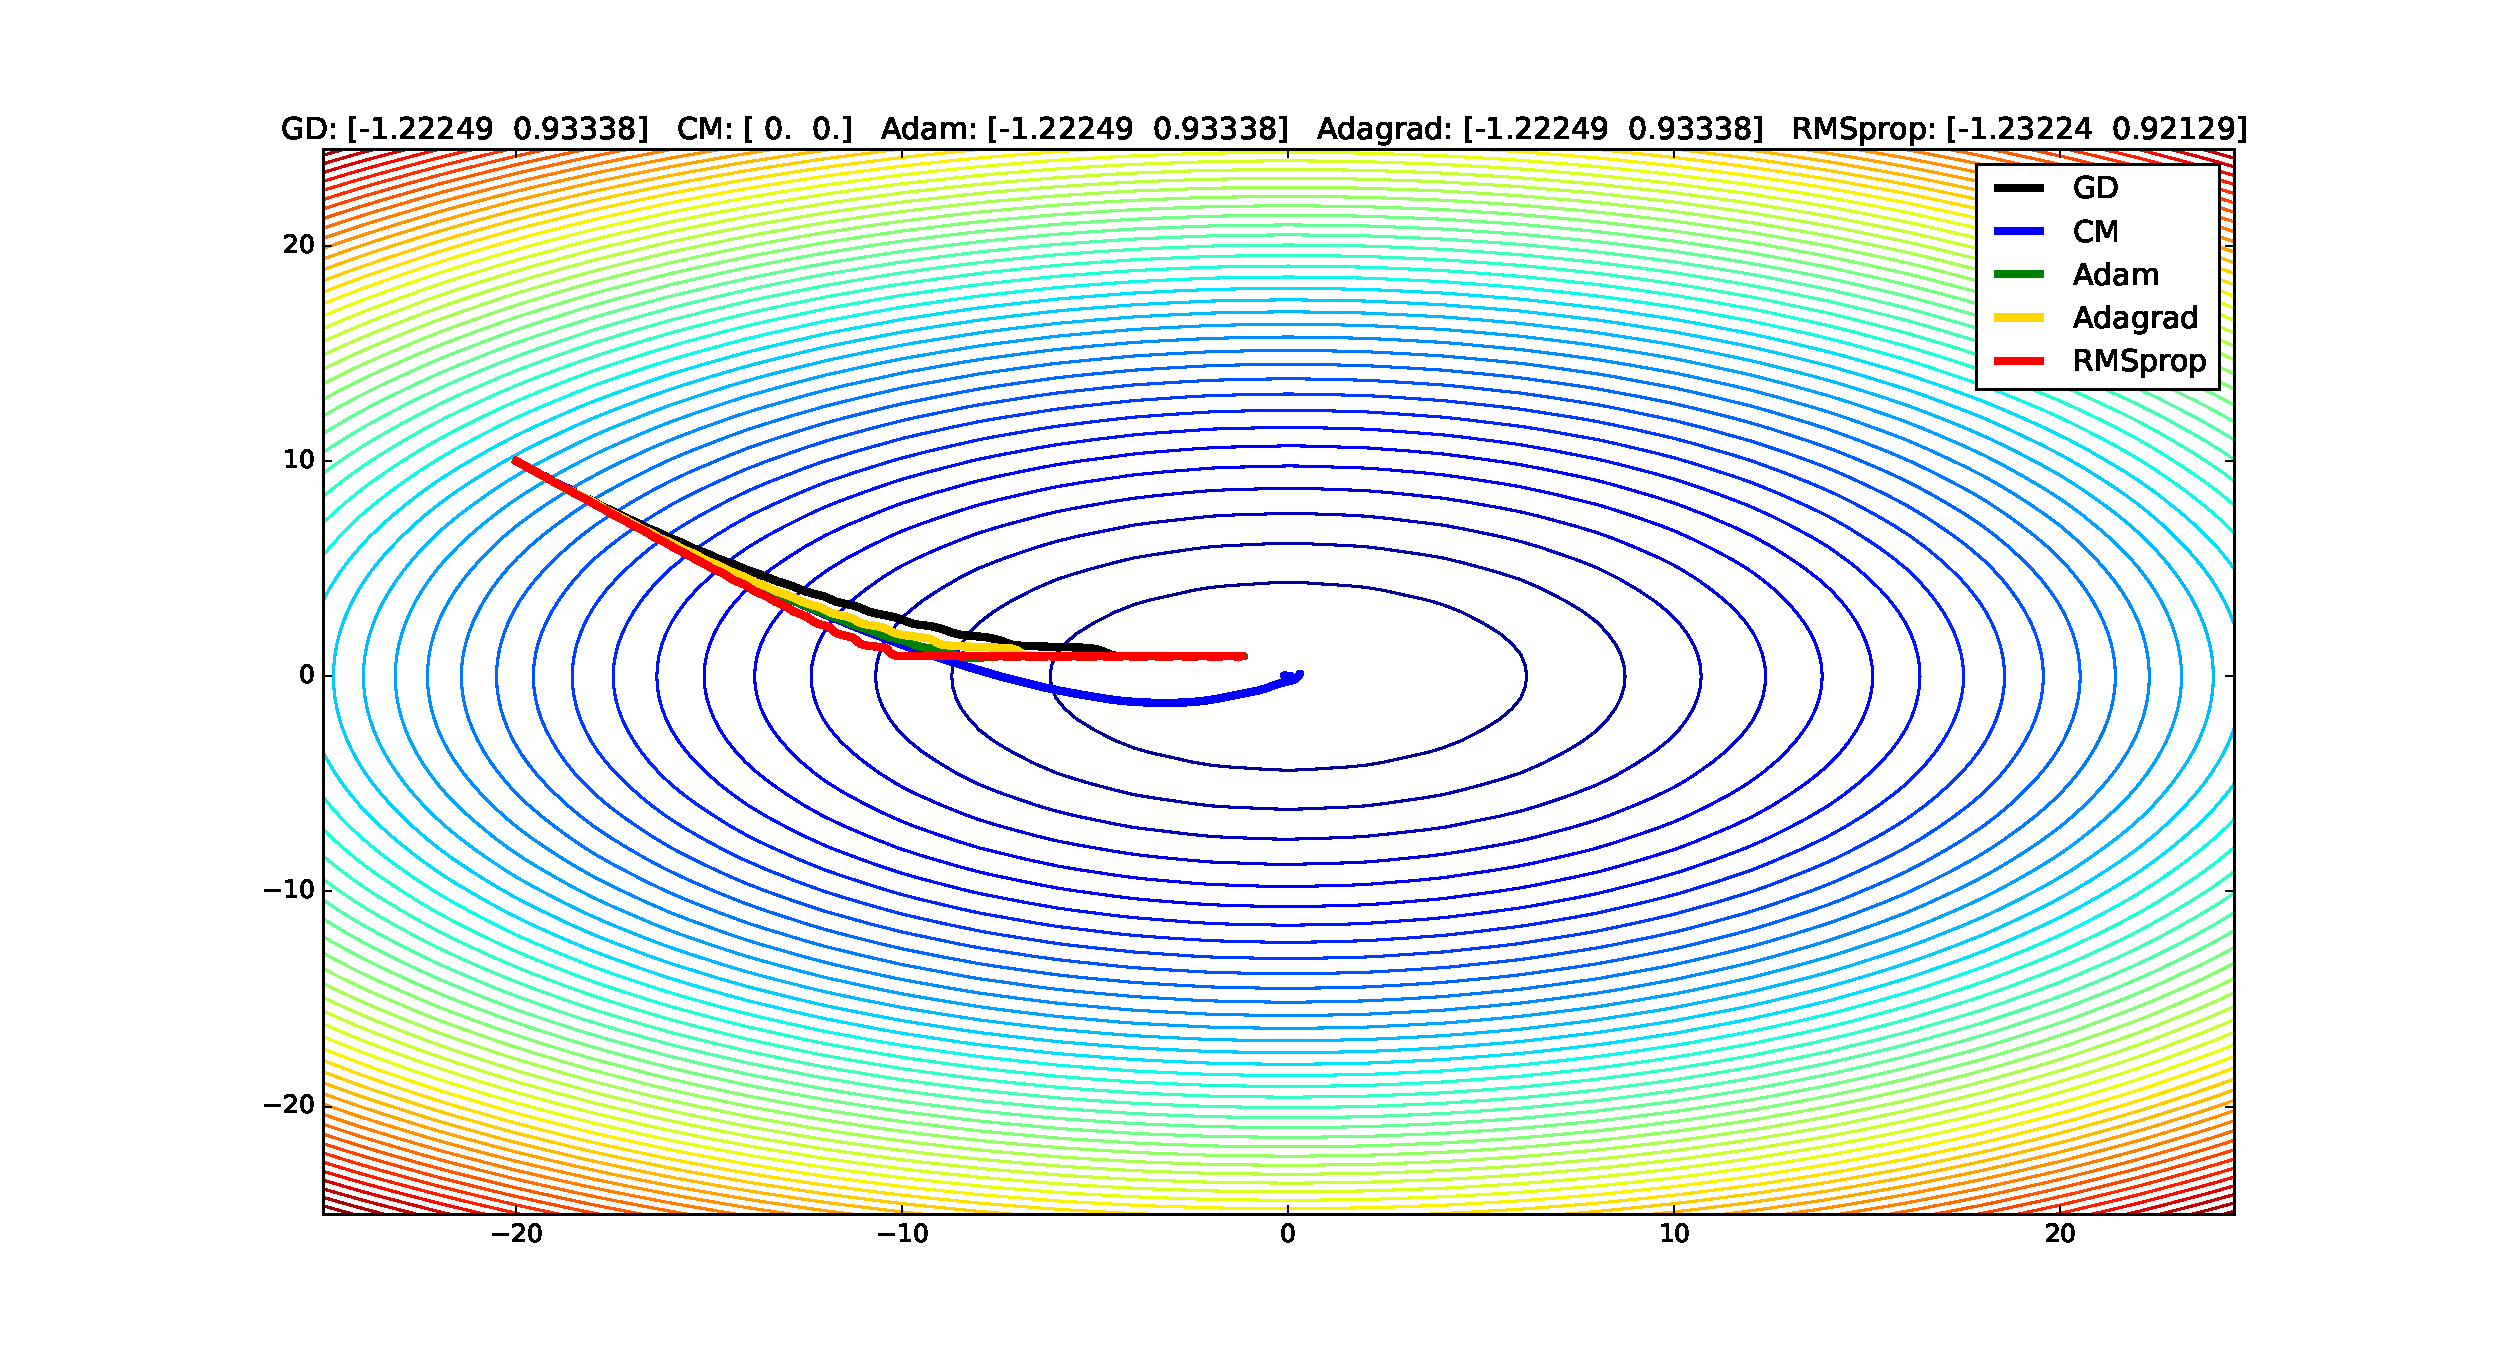
\includegraphics[width=\linewidth]{./images/B1.eps}
\end{figure}
\end{frame}

\begin{frame}{Behaviour with Bohachevsky's Function 2}
\begin{equation}
\label{B2}
f(\xbold) = x_{1}^{2} + 2x_{2}^{2} - 0.3\cos(3\pi x_{1})\cos(4\pi x_{2}) + 0.3
\end{equation}
\begin{figure}
\centering
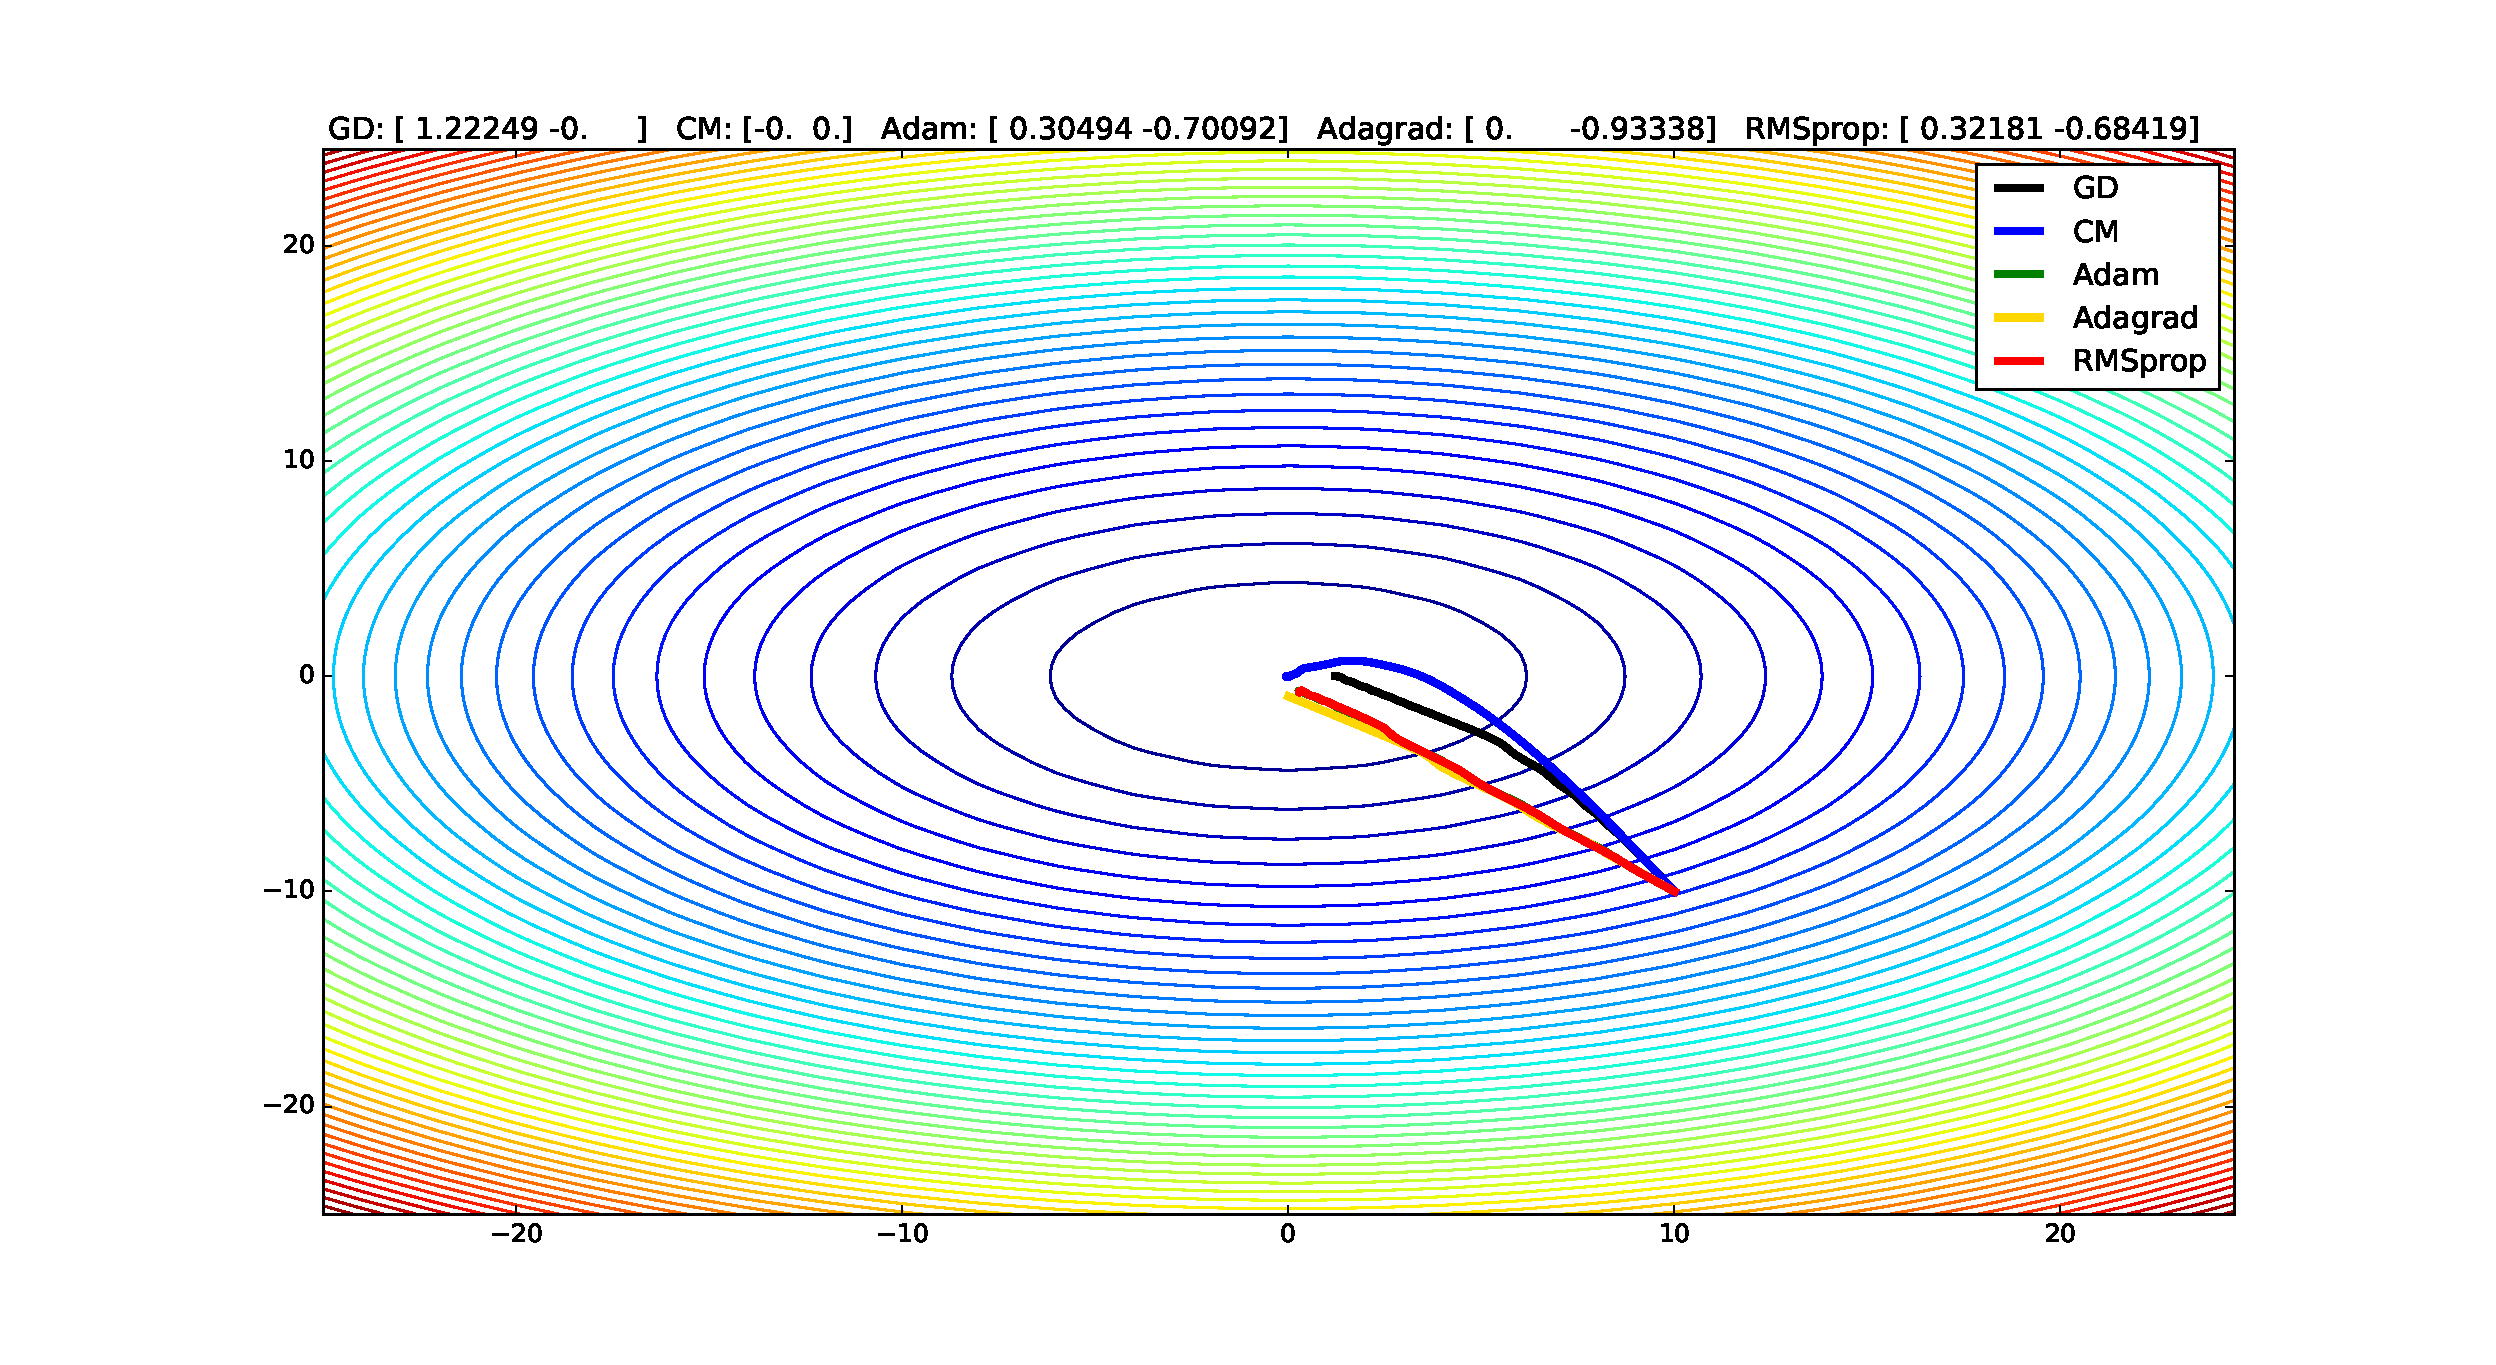
\includegraphics[width=\linewidth]{./images/B2.eps}
\end{figure}
\end{frame}

\begin{frame}{Behaviour with Bohachevsky's Function 3}
\begin{equation}
\label{B3}
f(\xbold) = x_{1}^{2} + 2x_{2}^{2} - 0.3\cos(3\pi x_{1} + 4\pi x_{2}) + 0.3
\end{equation}
\begin{figure}
\centering
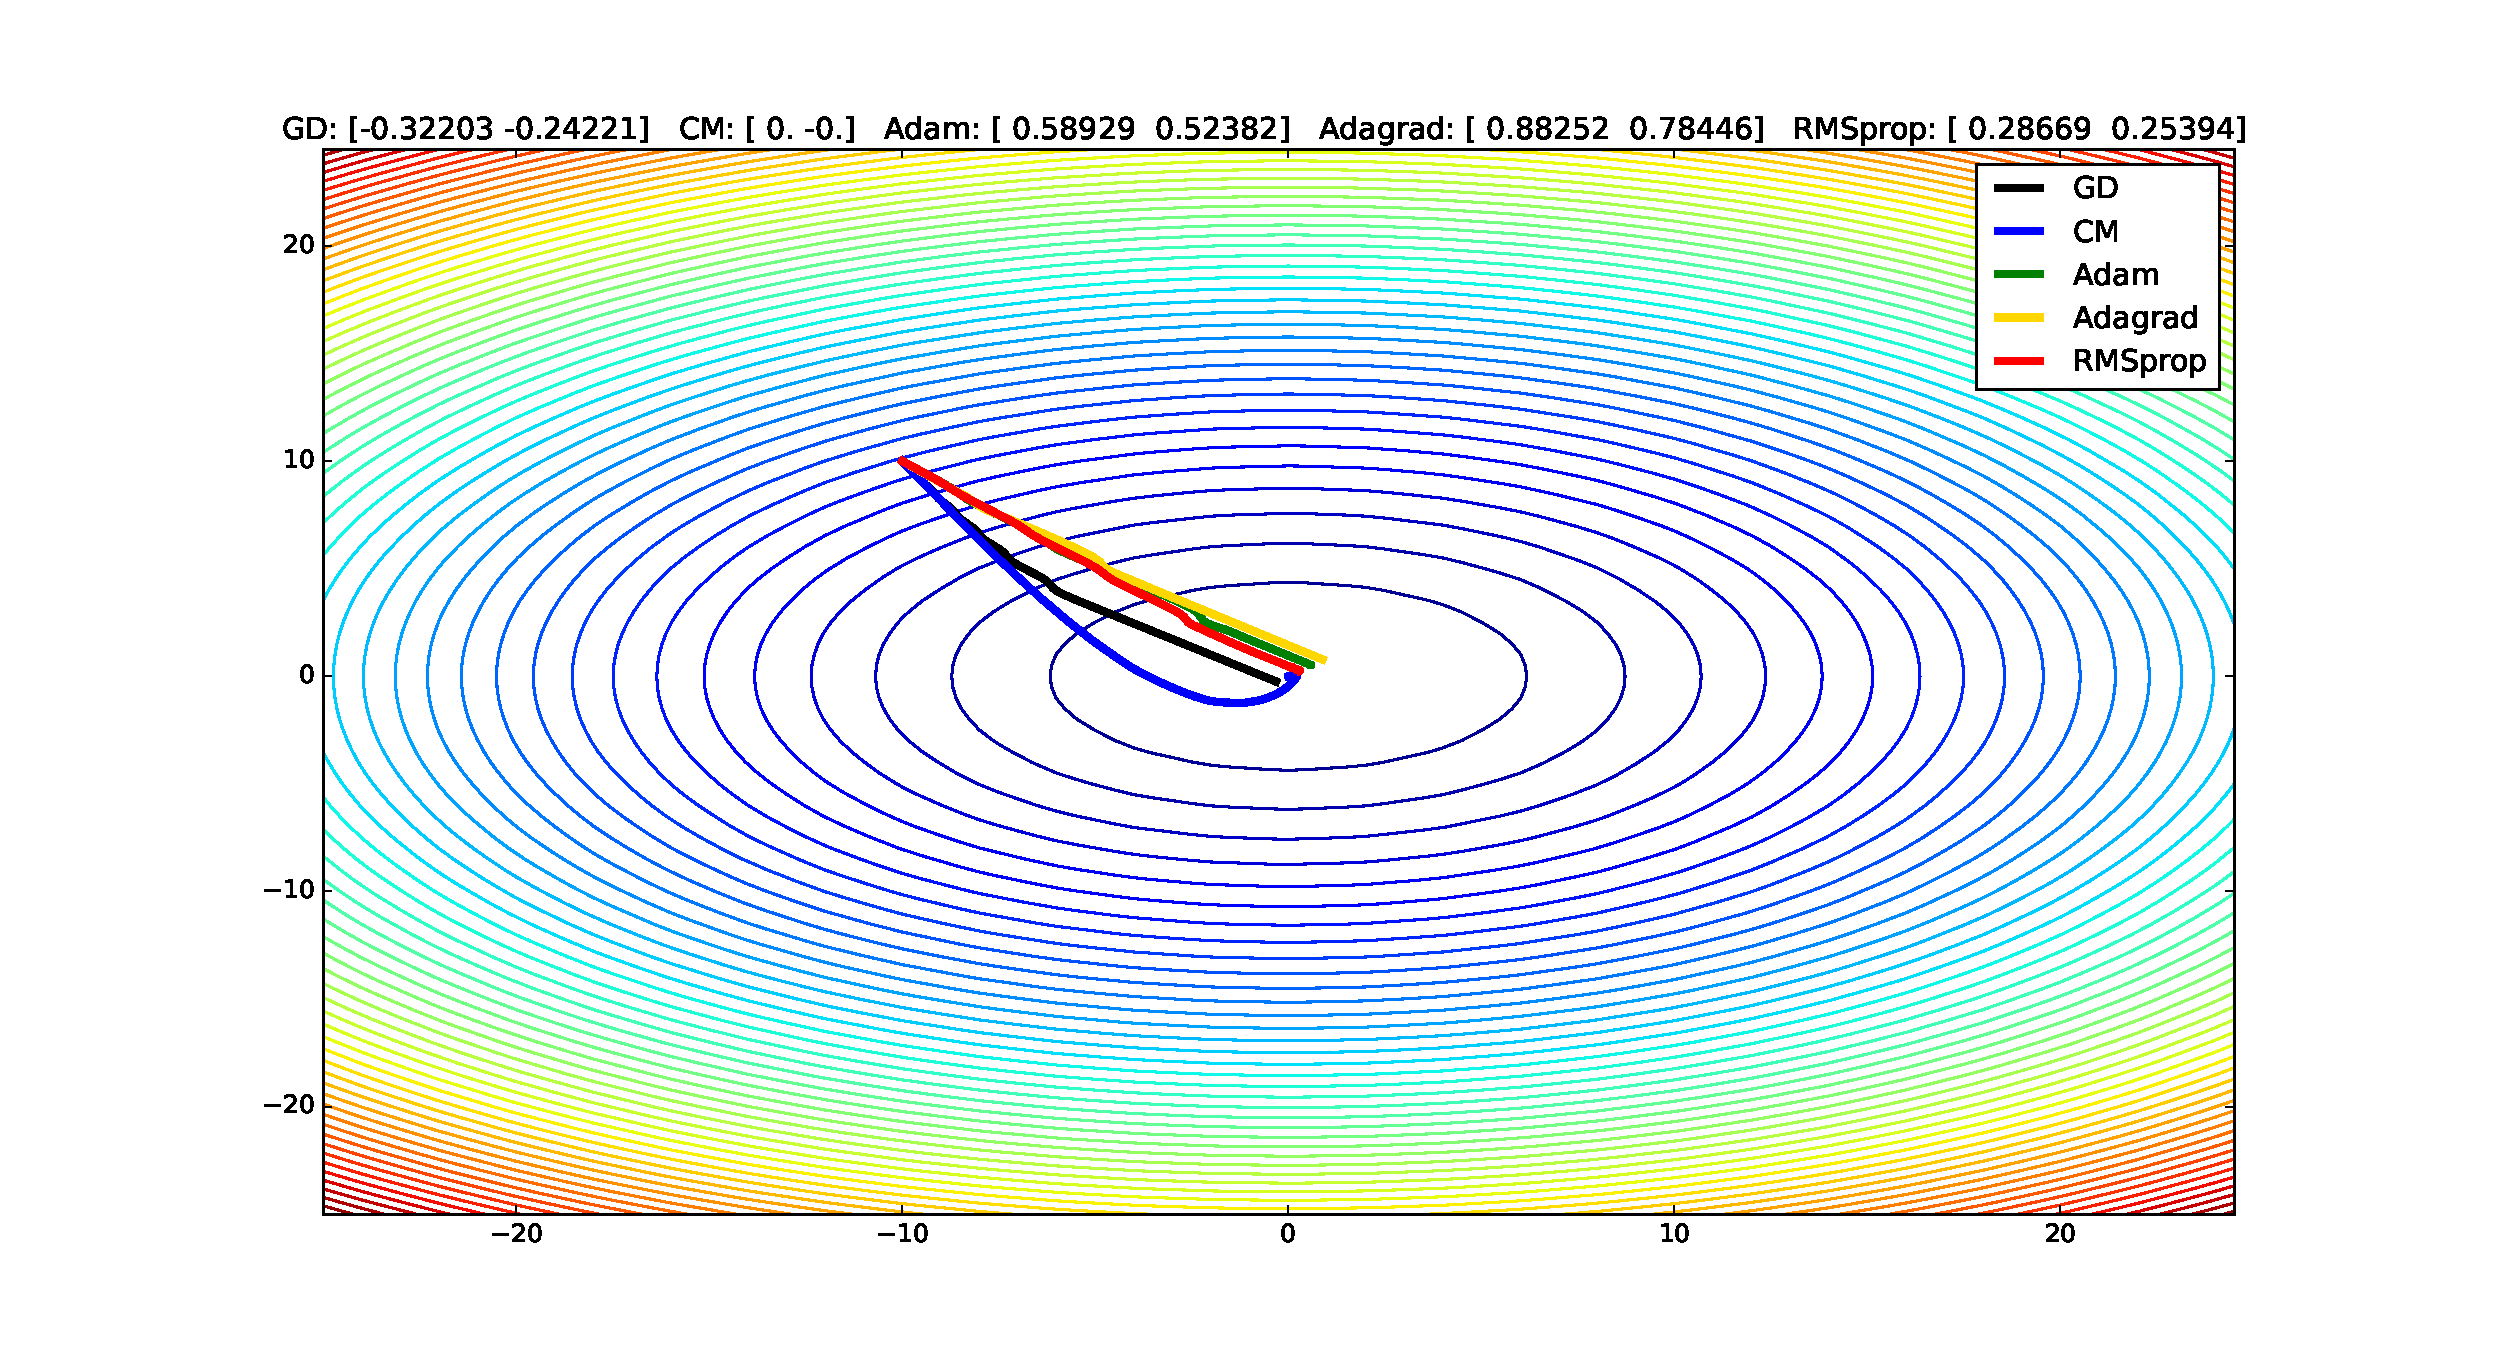
\includegraphics[width=\linewidth]{./images/B3.eps}
\end{figure}
\end{frame}

\begin{frame}{Behaviour with Beale's Function}
\begin{equation}
\label{BL}
f(\xbold) = (1.5 - x_{1} + x_{1}x_{2})^{2} + (2.25 - x_{1} + x_{1}x_{2}^{2})^{2} + (2.625 - x_{1} + x_{1}x_{2}^{3})^{2}
\end{equation}
\begin{figure}
\centering
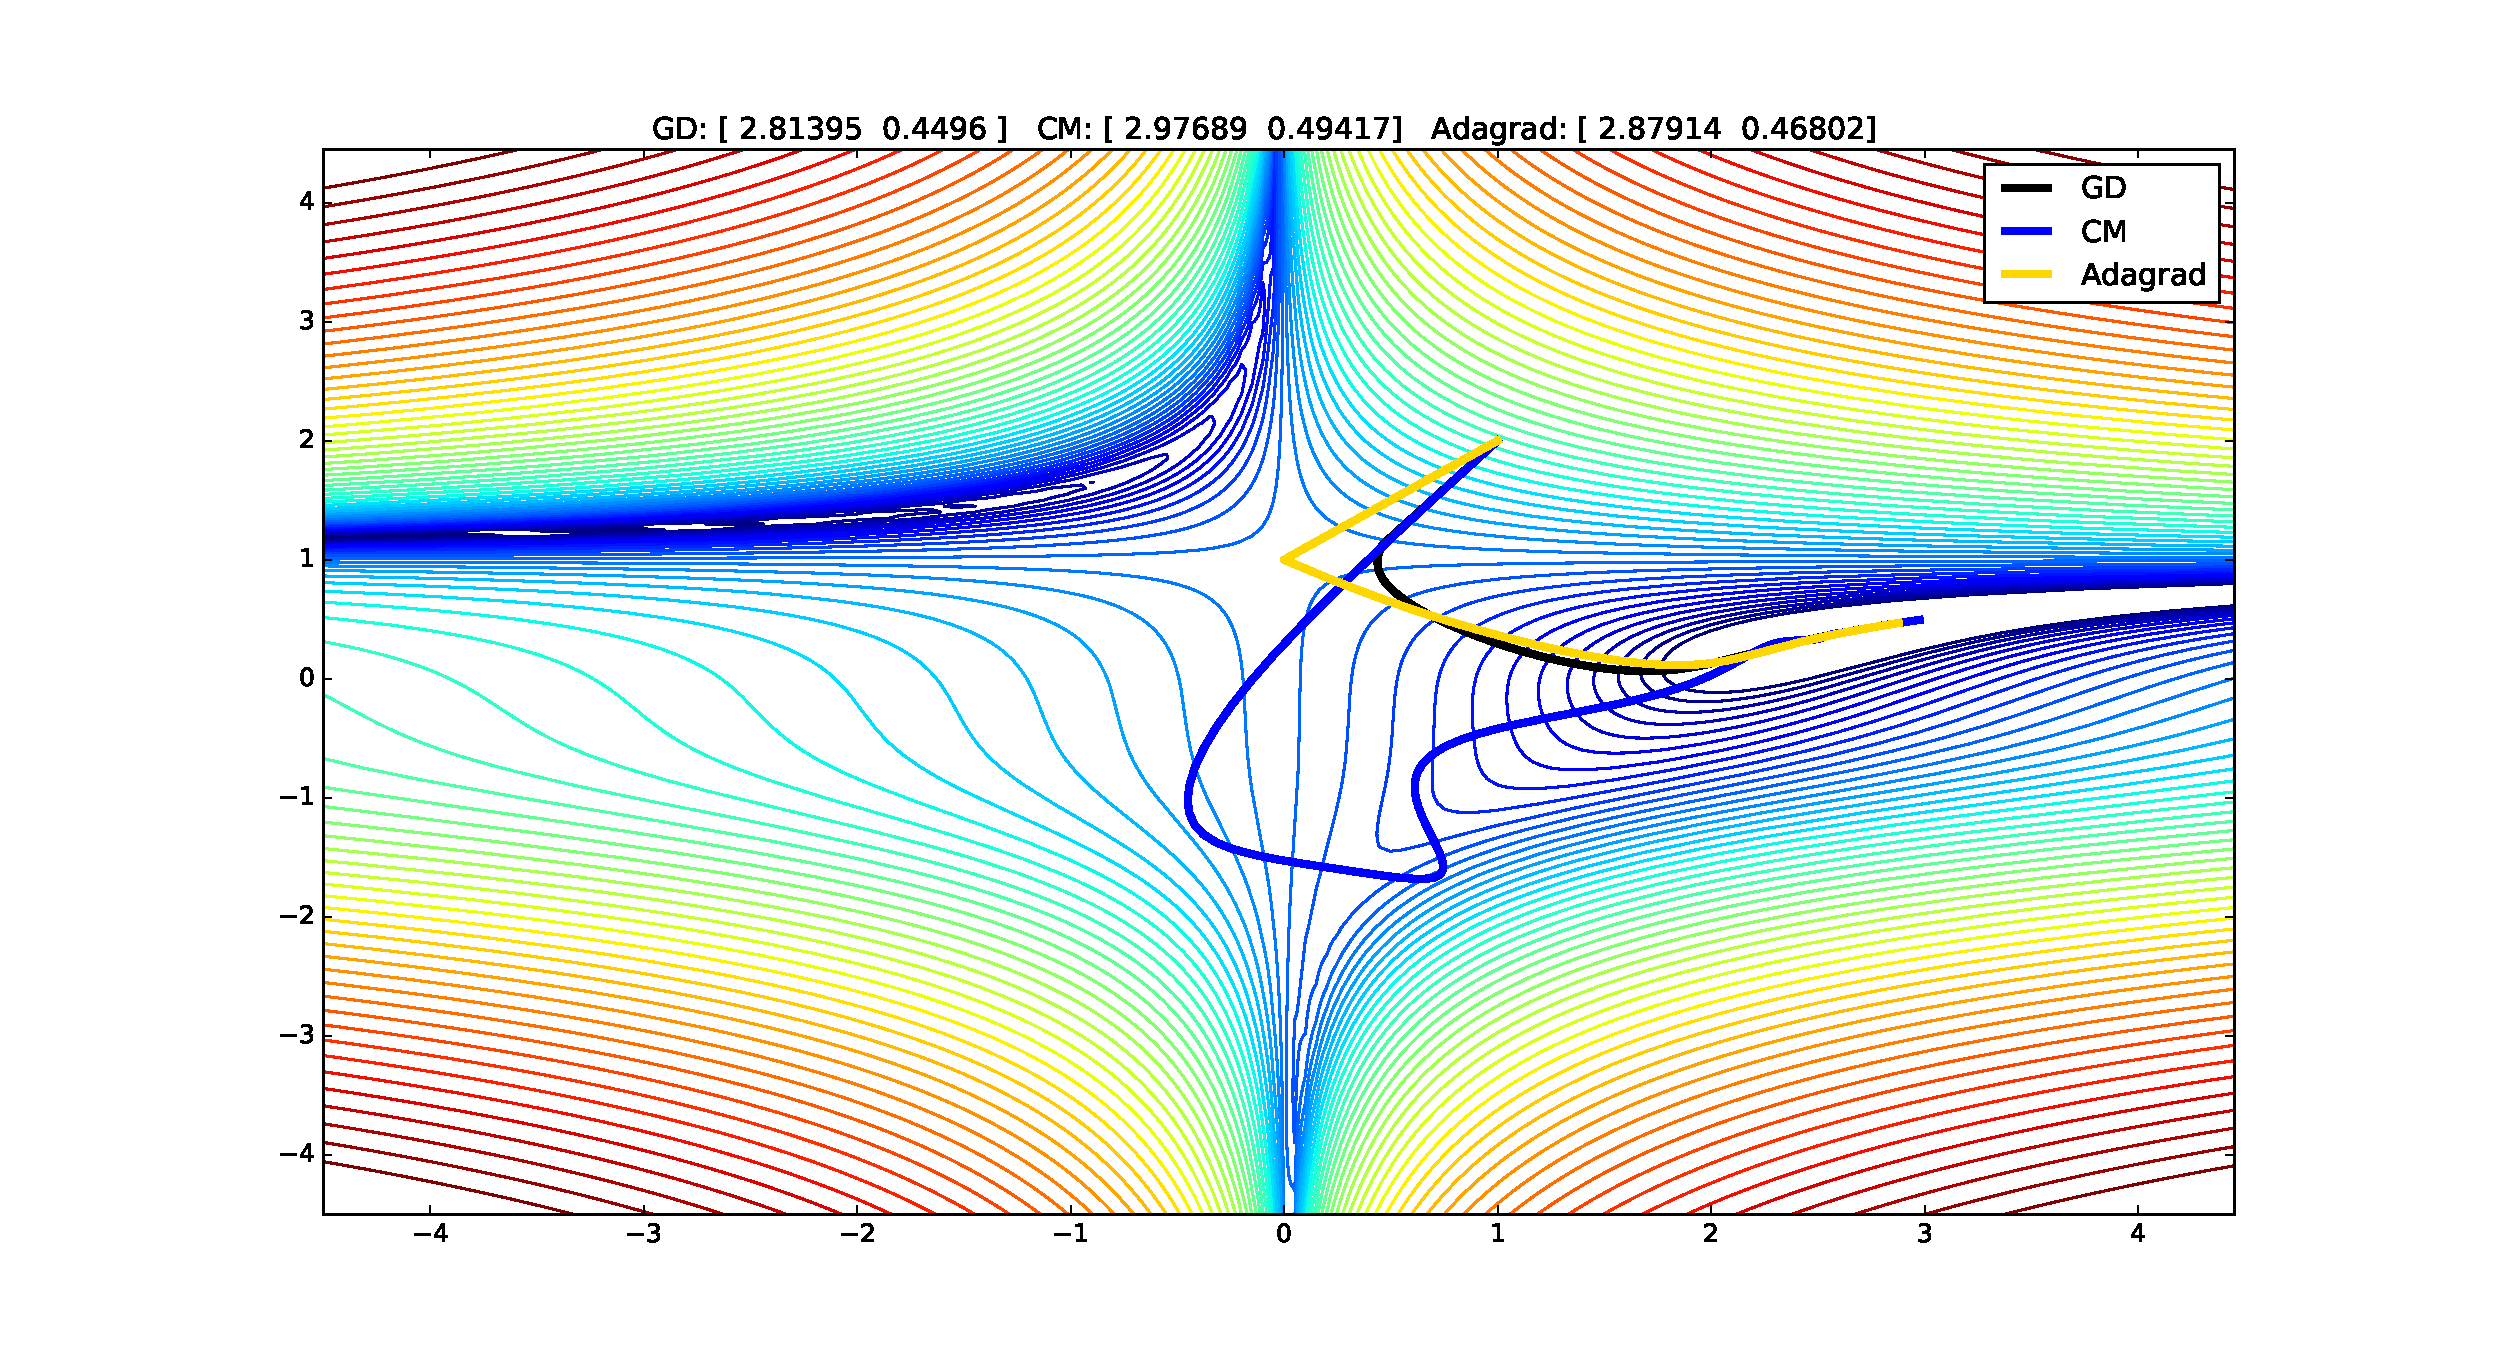
\includegraphics[width=\linewidth]{./images/BL.eps}
\end{figure}
\end{frame}

\begin{frame}{Behaviour with Rosenbrock's Function}
\begin{equation}
\label{RB}
f(\xbold;a=1, b=25) = (1 - x_{1})^{2} + 25(x_{2} - x_{1})^{2}
\end{equation}
\begin{figure}
\centering
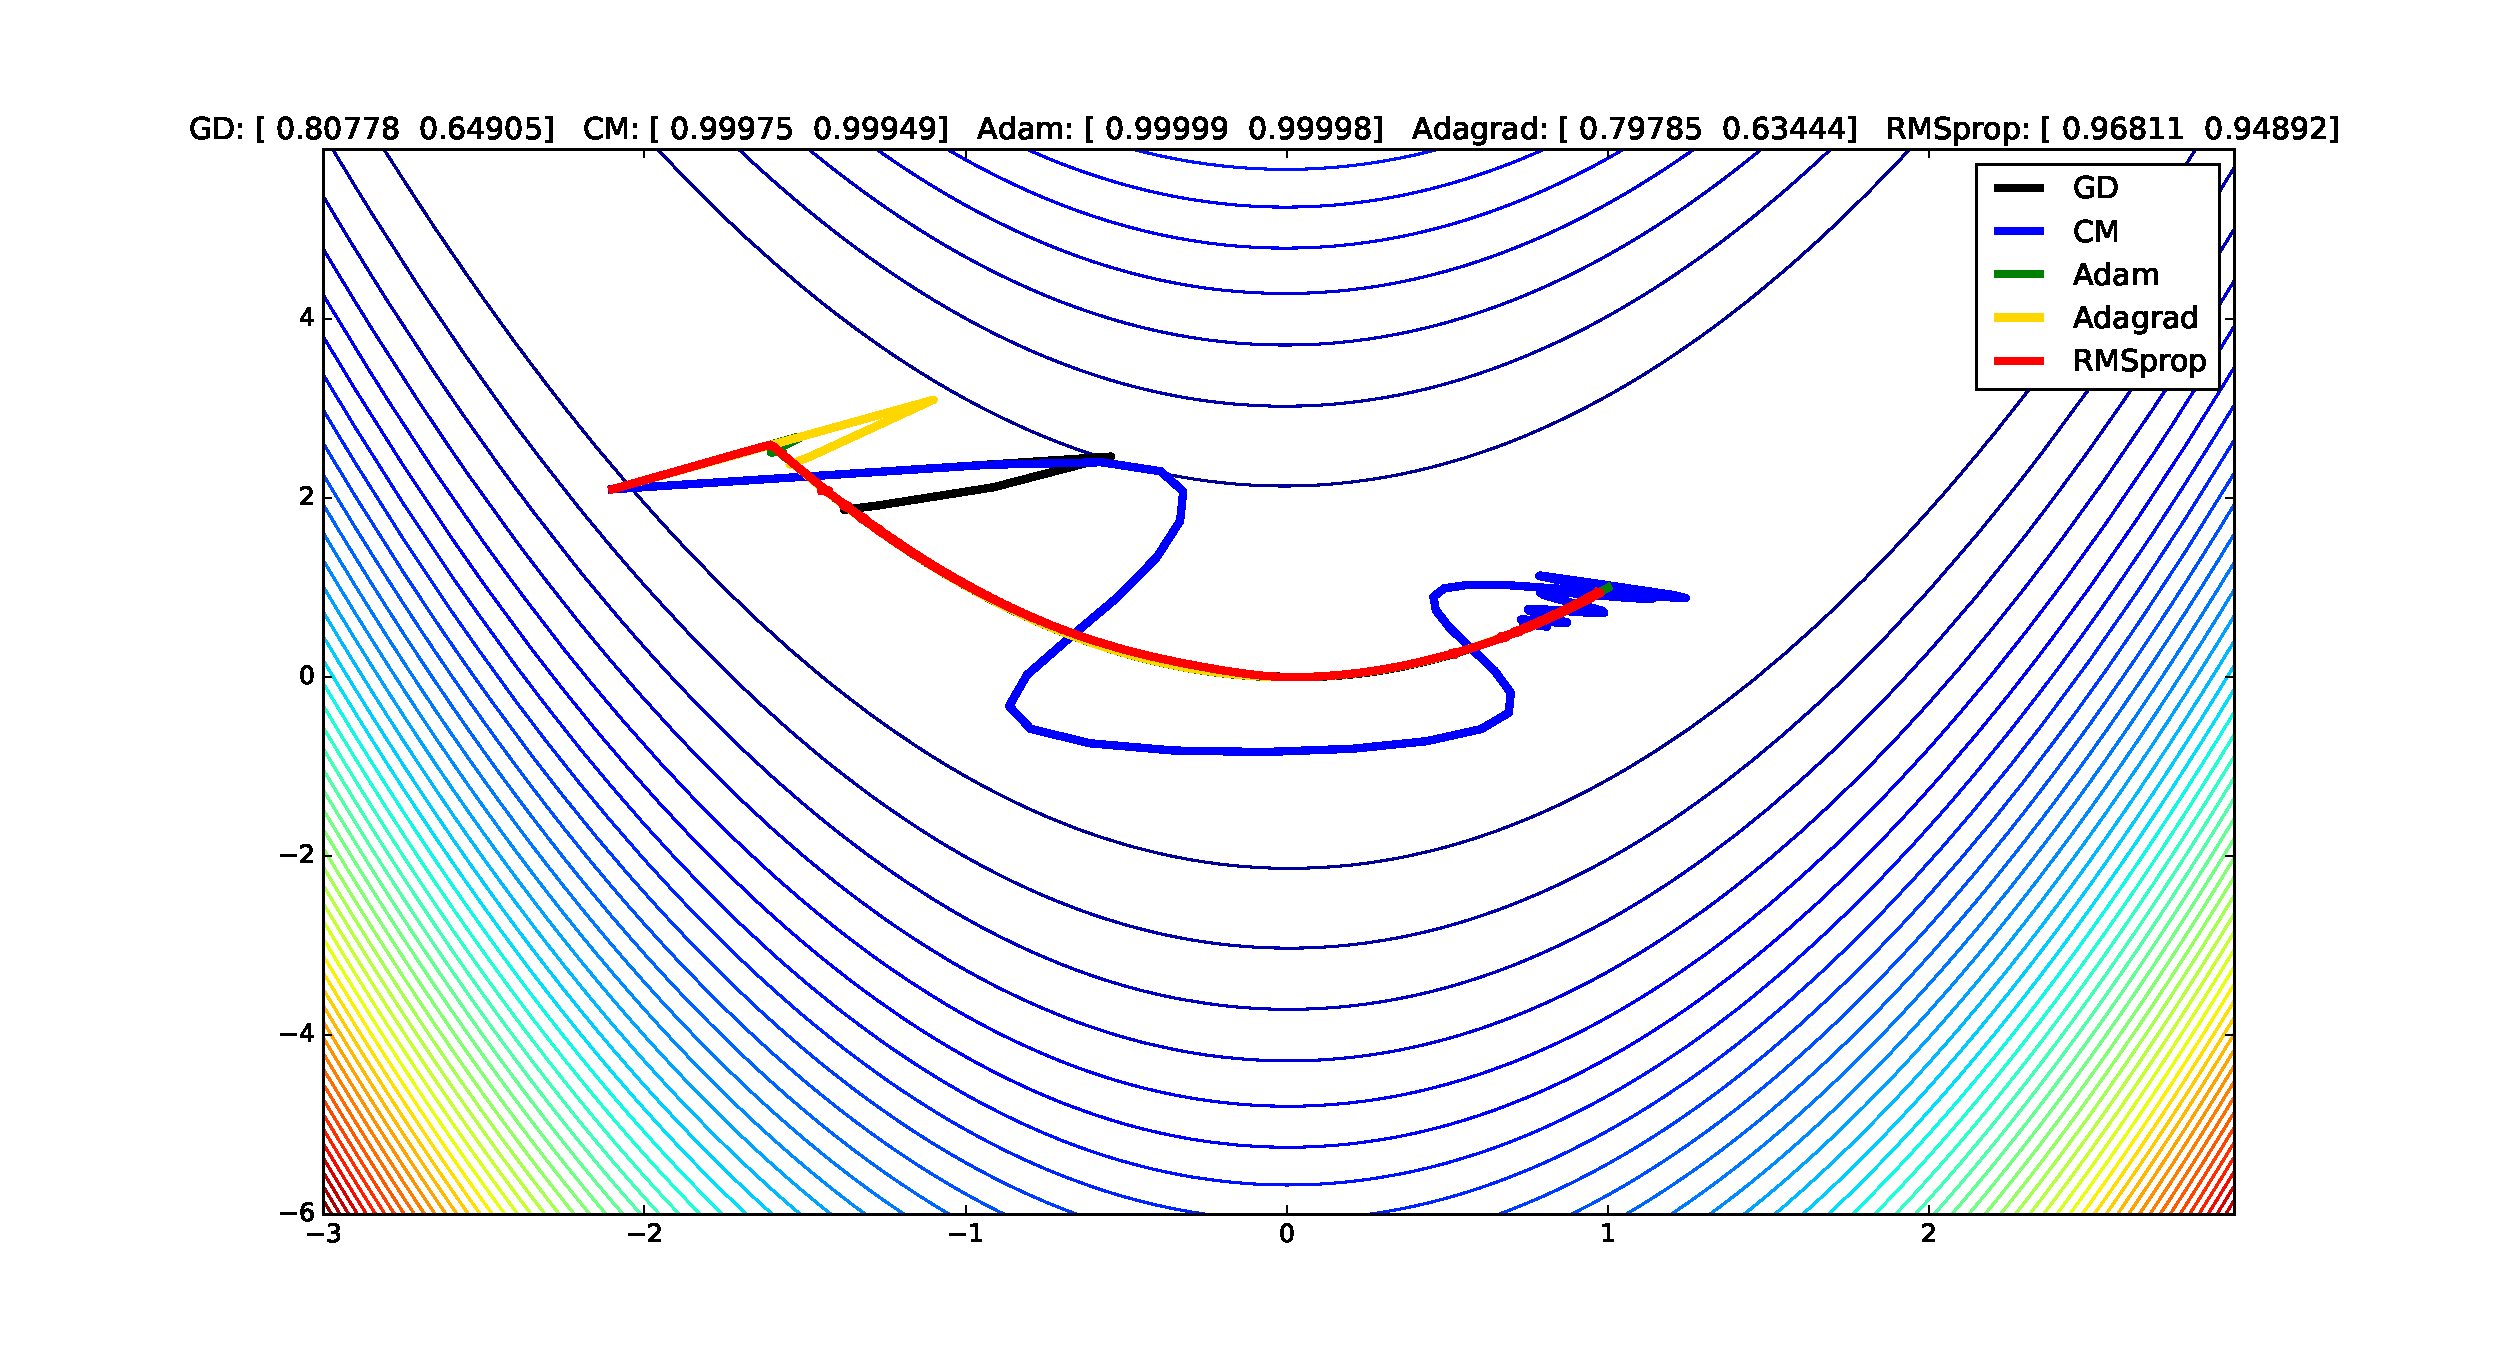
\includegraphics[width=\linewidth]{./images/RB.eps}
\end{figure}
\end{frame}

\subsection{Deep Learning Experiments: MLP Classifiers}
\begin{frame}{Multi-Layer Perceptron Classifiers}
\begin{itemize}
\item<1->{Took Multilayer perceptron classifiers for the MNIST\footnote{\url{http://yann.lecun.com/exdb/mnist/}} and CIFAR10\footnote{\url{https://www.cs.toronto.edu/~kriz/cifar.html}} datasets}
\item<2->{Achieved \(\approx 95\%\) on MNIST and \(\approx 60\%\) on CIFAR10
          \begin{itemize}
          \item<3->{Not State-of-the-art, only to analyze the behaviour of the optimization methods}
          \end{itemize}
         }
\item<3->{Activation used between the layers was \texttt{ReLU}}
\item<4->{Trained for 10000 iterations, chose optimal learning rate from \(\{0.5, 0.2, 0.1, 0.05, 0.02, 0.01, 0.005, 0.002, 0.001, 0.0005, 0.0002, 0.0001\}\)}
\end{itemize}
\end{frame}

\begin{frame}{MNIST with Architecture: \texttt{784-500-500-500-10} - Training Loss vs Mini-batches}
\begin{figure}
\centering
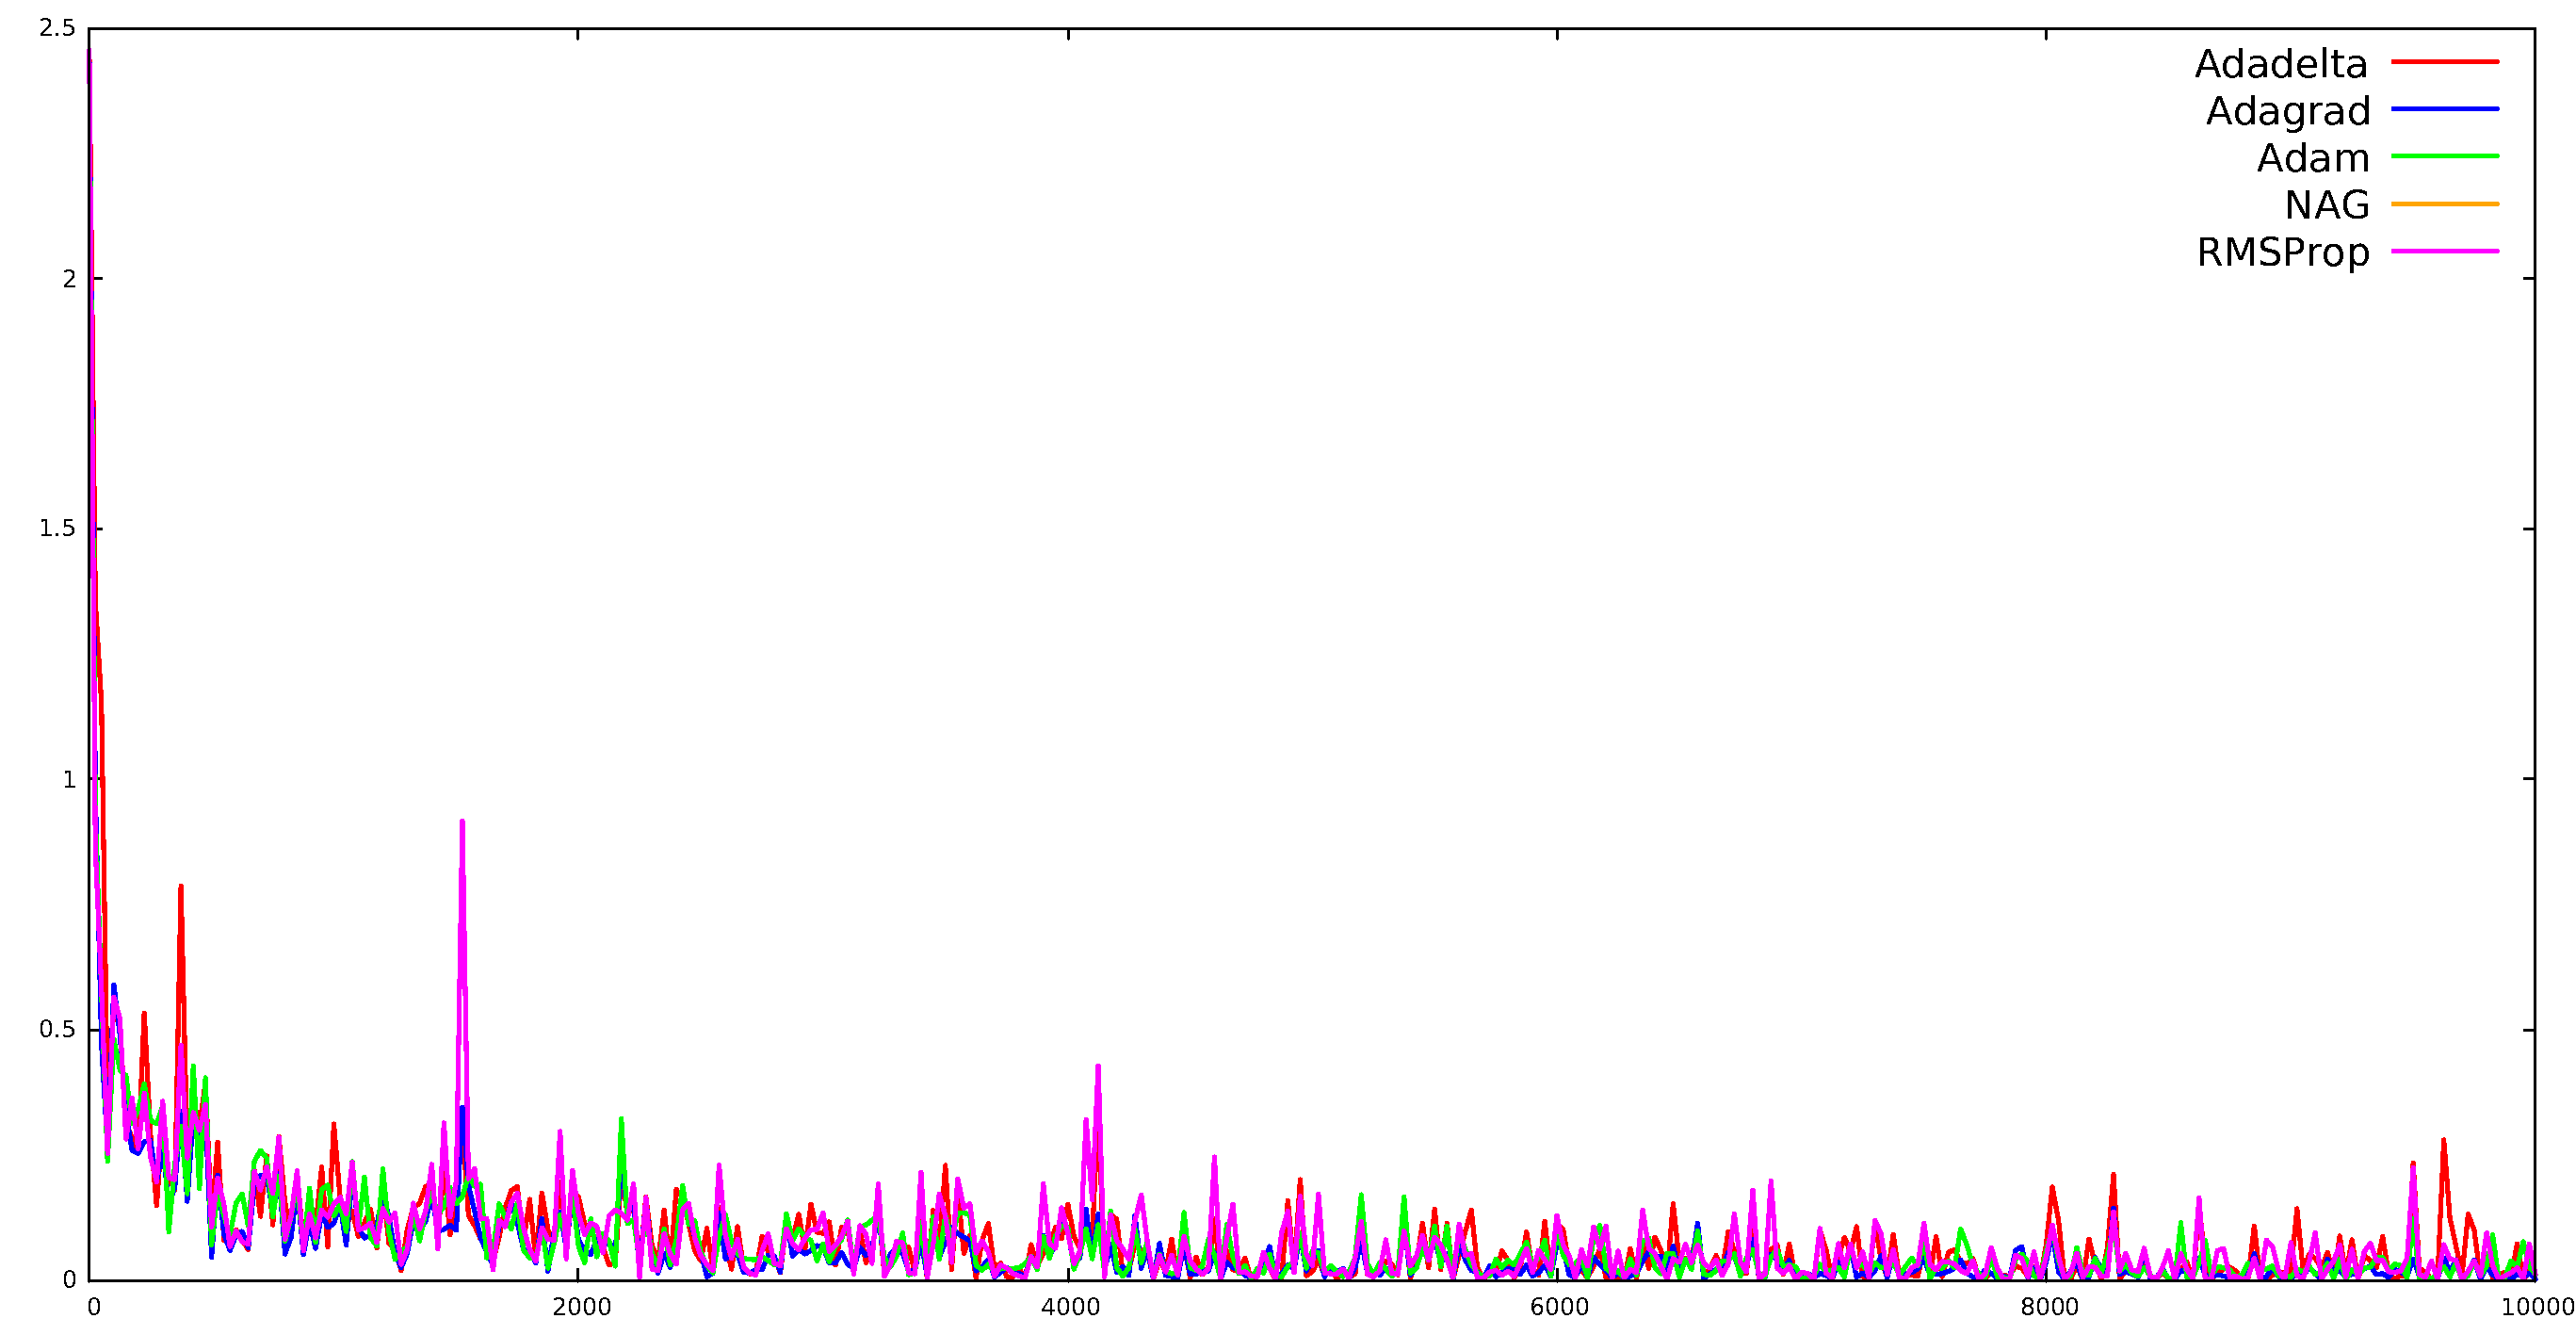
\includegraphics[width=\linewidth]{./images/mnist-1.pdf}
\end{figure}
\end{frame}

\begin{frame}{MNIST with Architecture: \texttt{784-1000-1000-1000-10} - Training Loss vs Mini-batches}
\begin{figure}
\centering
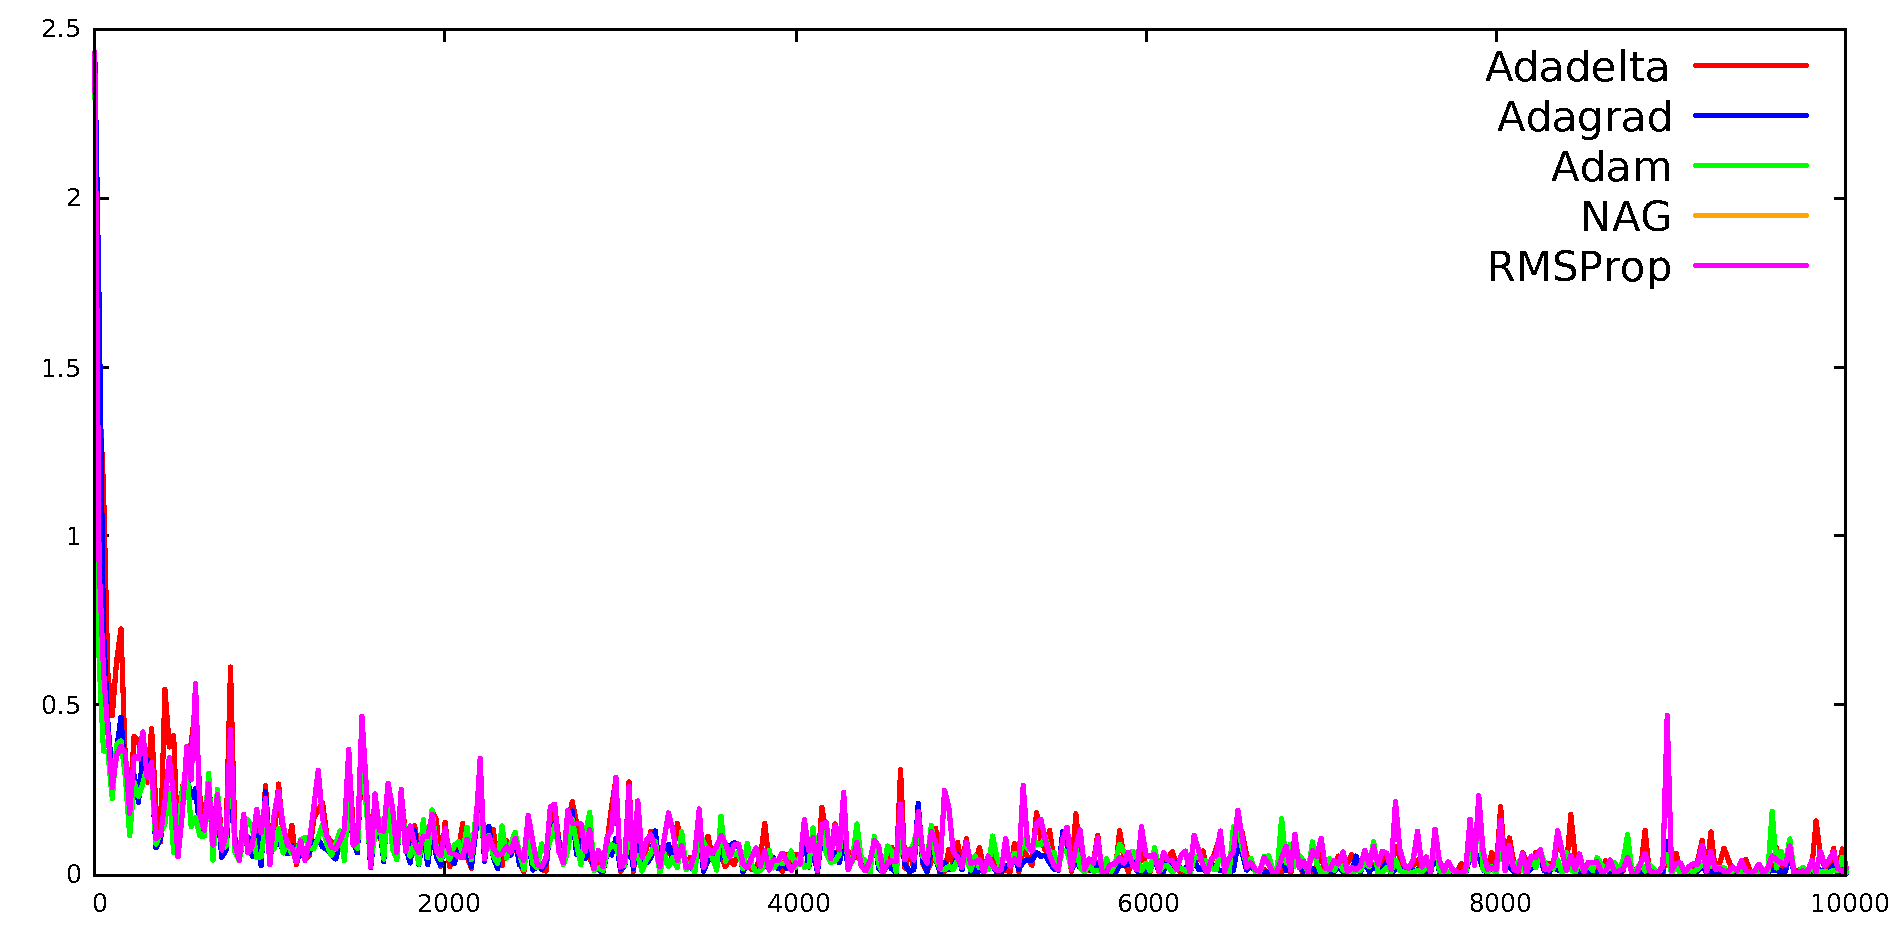
\includegraphics[width=\linewidth]{./images/mnist-2.pdf}
\end{figure}
\end{frame}

\begin{frame}{CIFAR10 with Architecture: \texttt{3072-1000-500-10} - Training Loss vs Mini-batches}
\begin{figure}
\centering
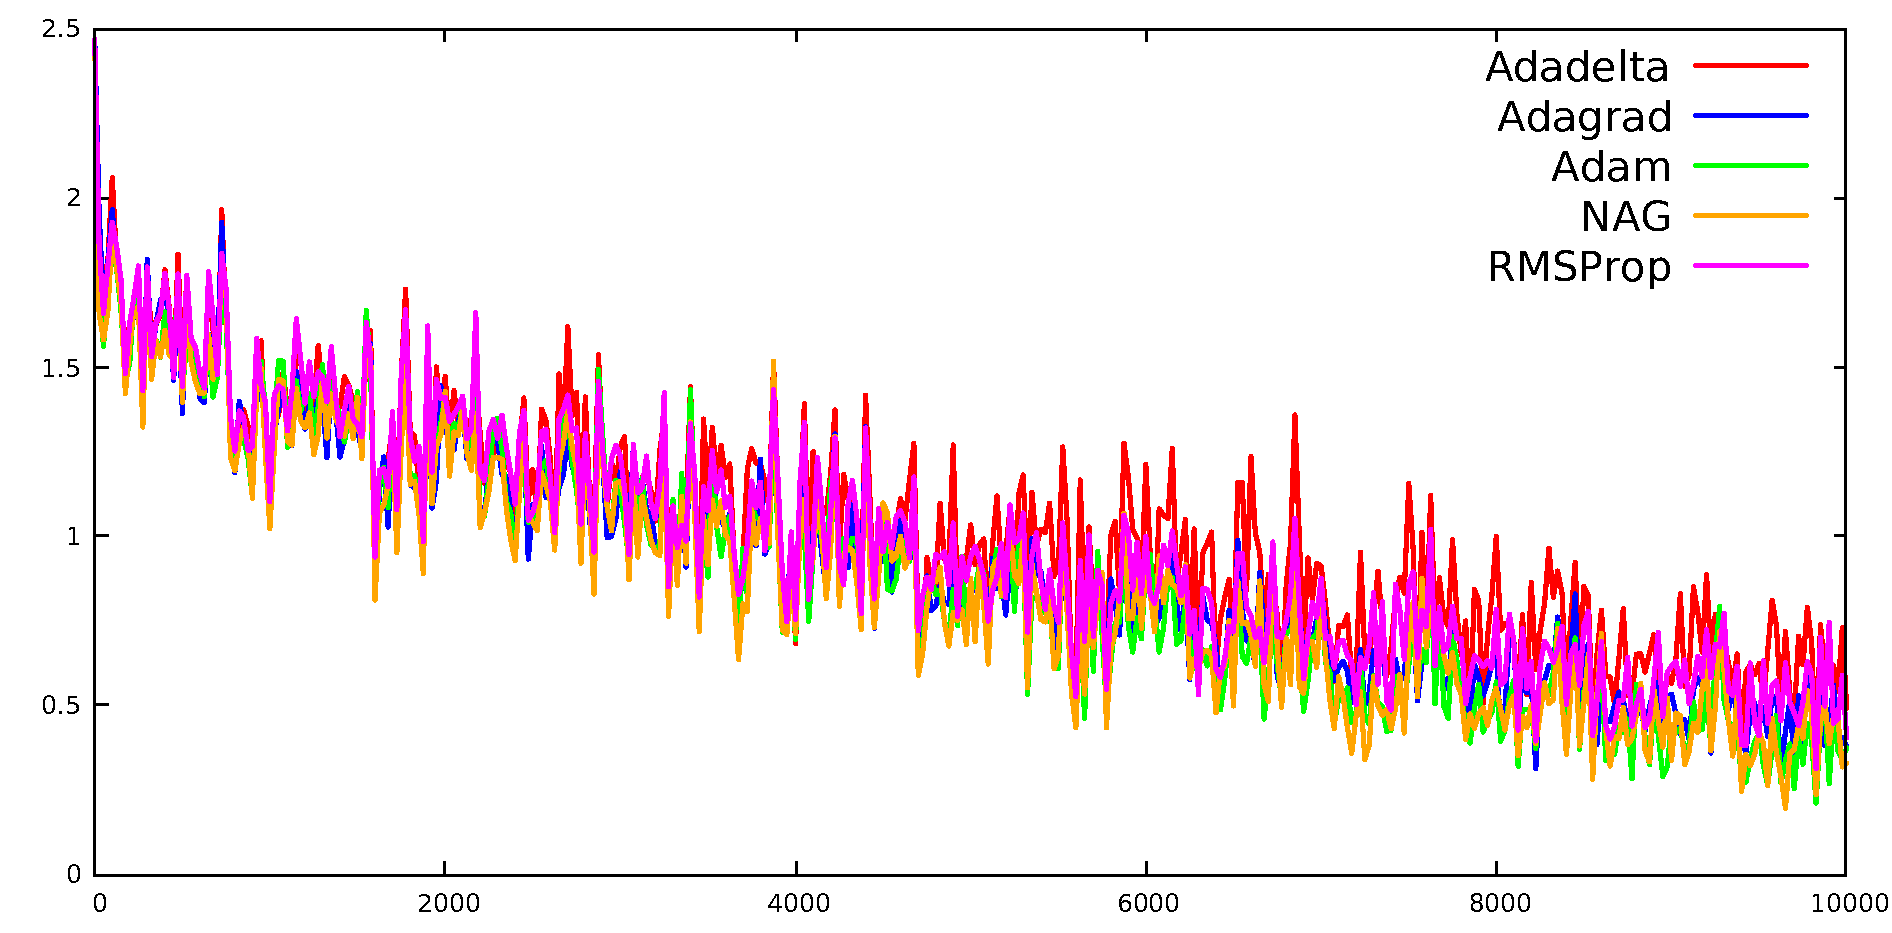
\includegraphics[width=\linewidth]{./images/cifar10-1.pdf}
\end{figure}
\end{frame}

\begin{frame}{CIFAR10 with Architecture: \texttt{3072-1000-1000-1000-10} - Training Loss vs Mini-batches}
\begin{figure}
\centering
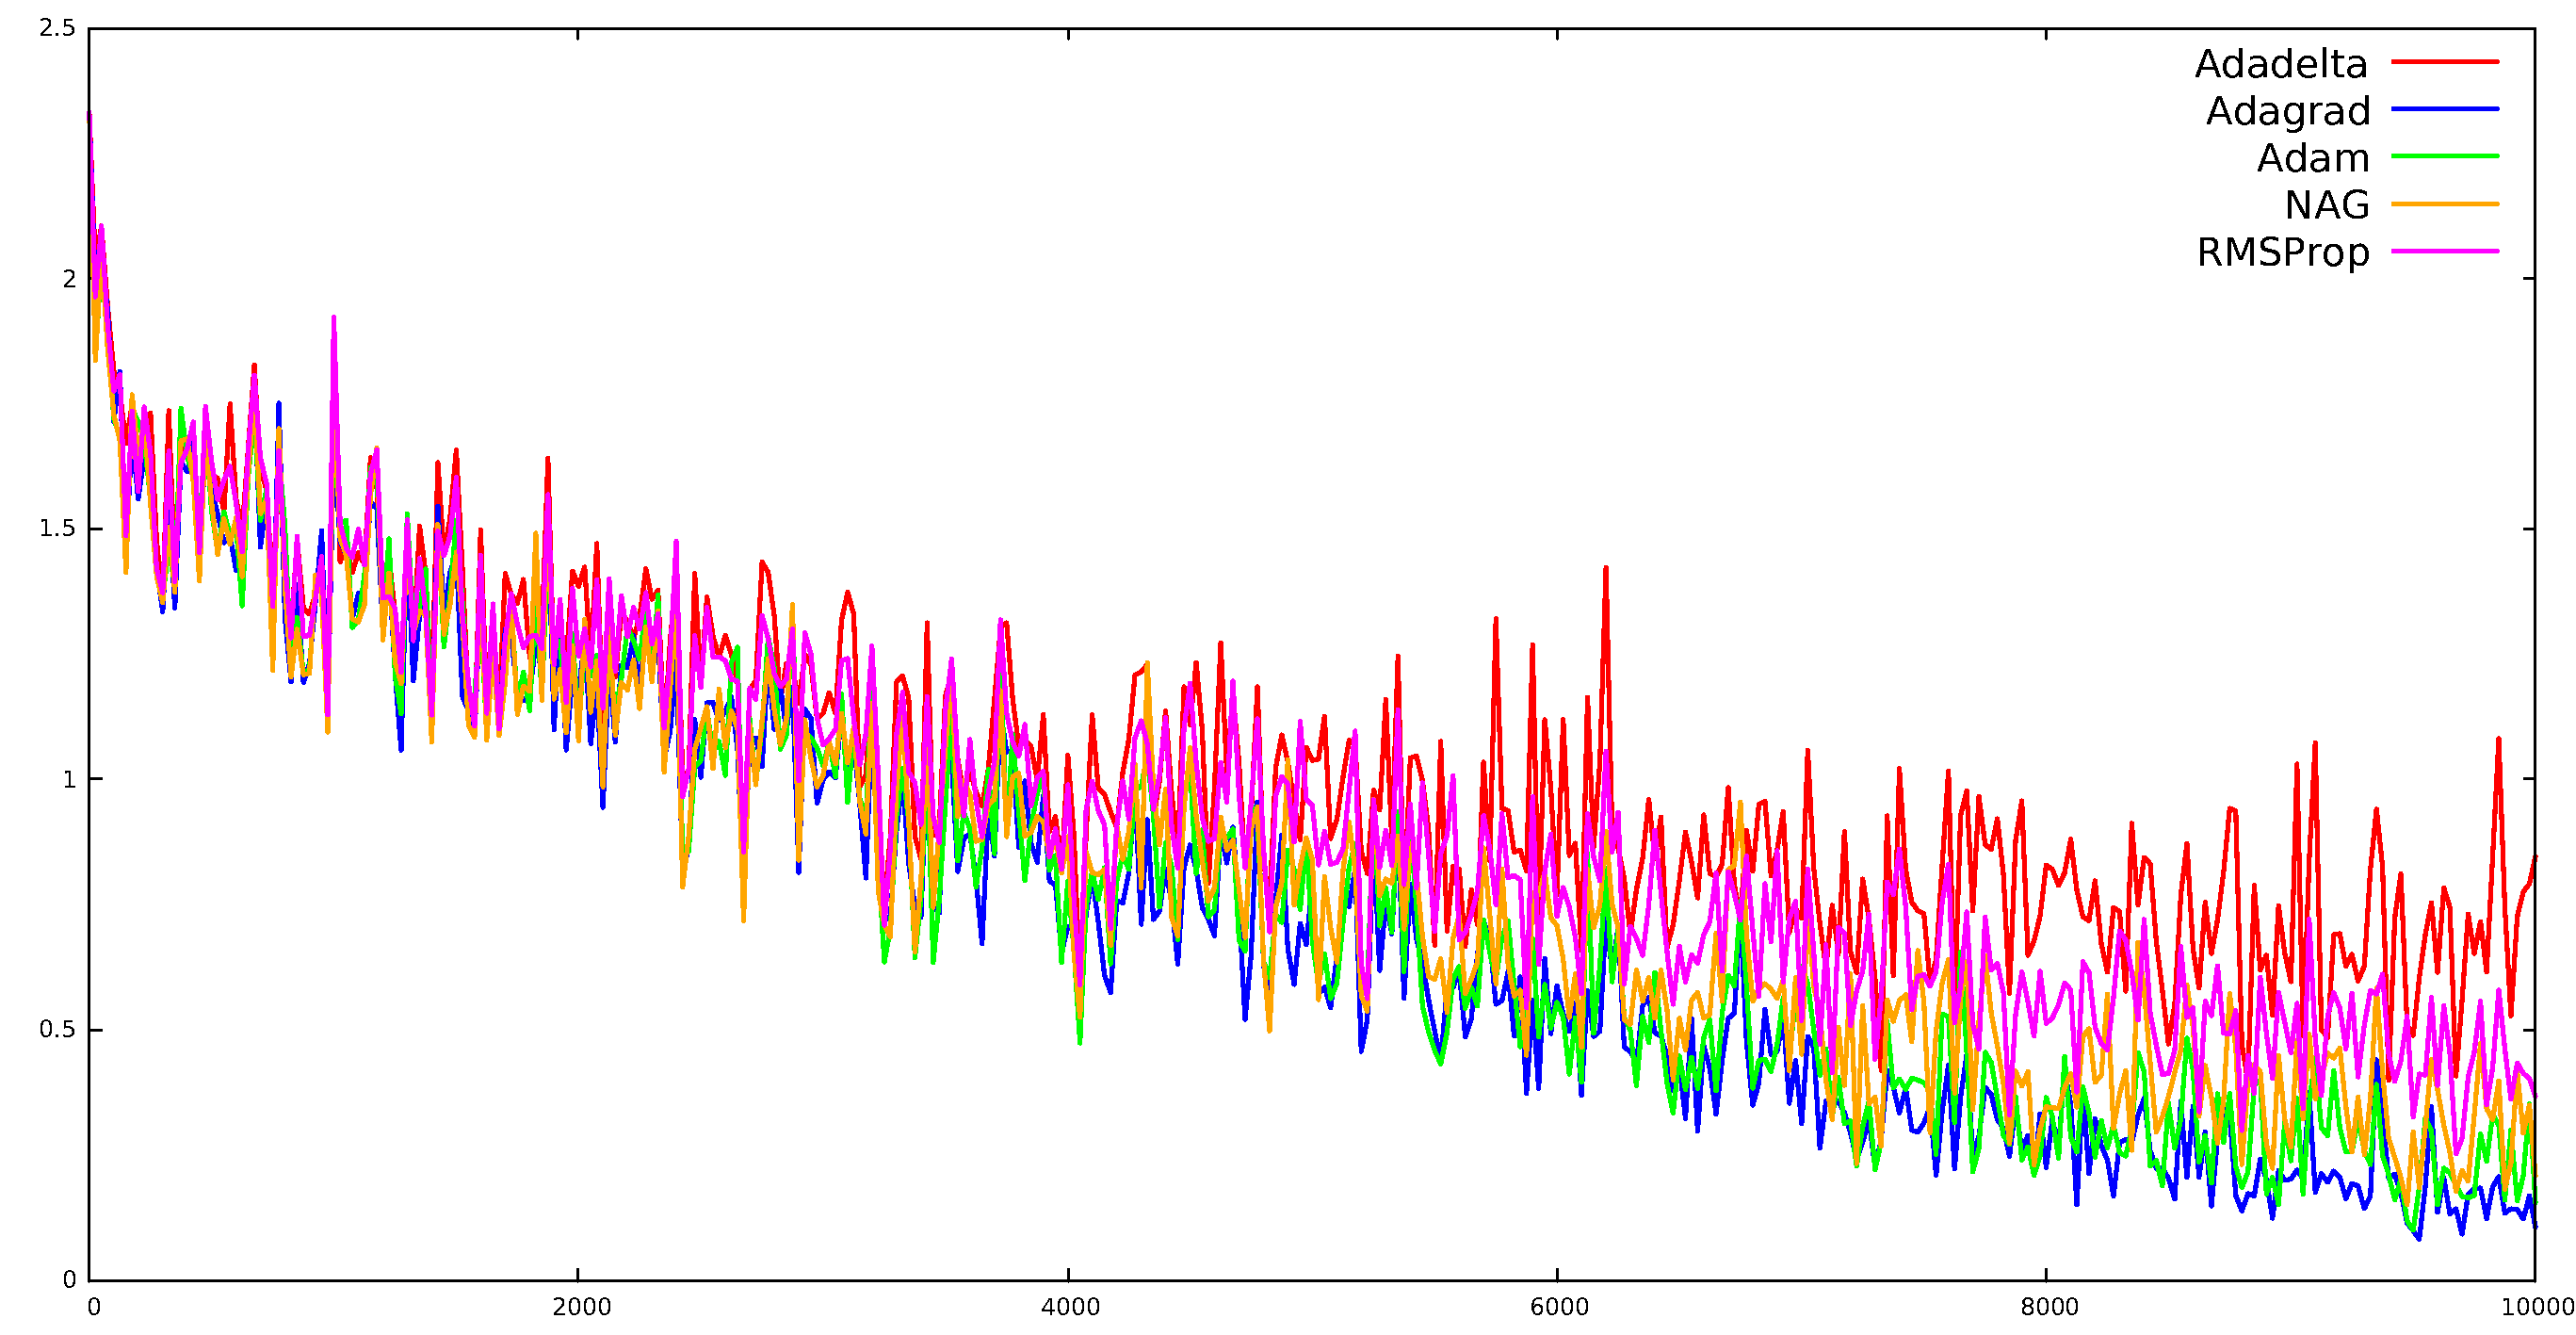
\includegraphics[width=\linewidth]{./images/cifar10-2.pdf}
\end{figure}
\end{frame}

\subsection{Deep Learning Experiments: Autoencoders}
\begin{frame}{Deep Autoencoders}
\begin{itemize}
\item<1->{Used a multilayer perceptron deep autoencoder for encoding MNIST images}
\item<2->{Activation used between the layers was \texttt{sigmoid}}
\item<3->{Trained for 10000 iterations, chose optimal learning rate from \(\{0.5, 0.2, 0.1, 0.05, 0.02, 0.01, 0.005, 0.002, 0.001, 0.0005, 0.0002, 0.0001\}\)}
\end{itemize}
\end{frame}

\begin{frame}{Autoencoder architecture: \texttt{784-1000-500-1000-10} - Training Loss vs Mini-batches}
\begin{figure}
\centering
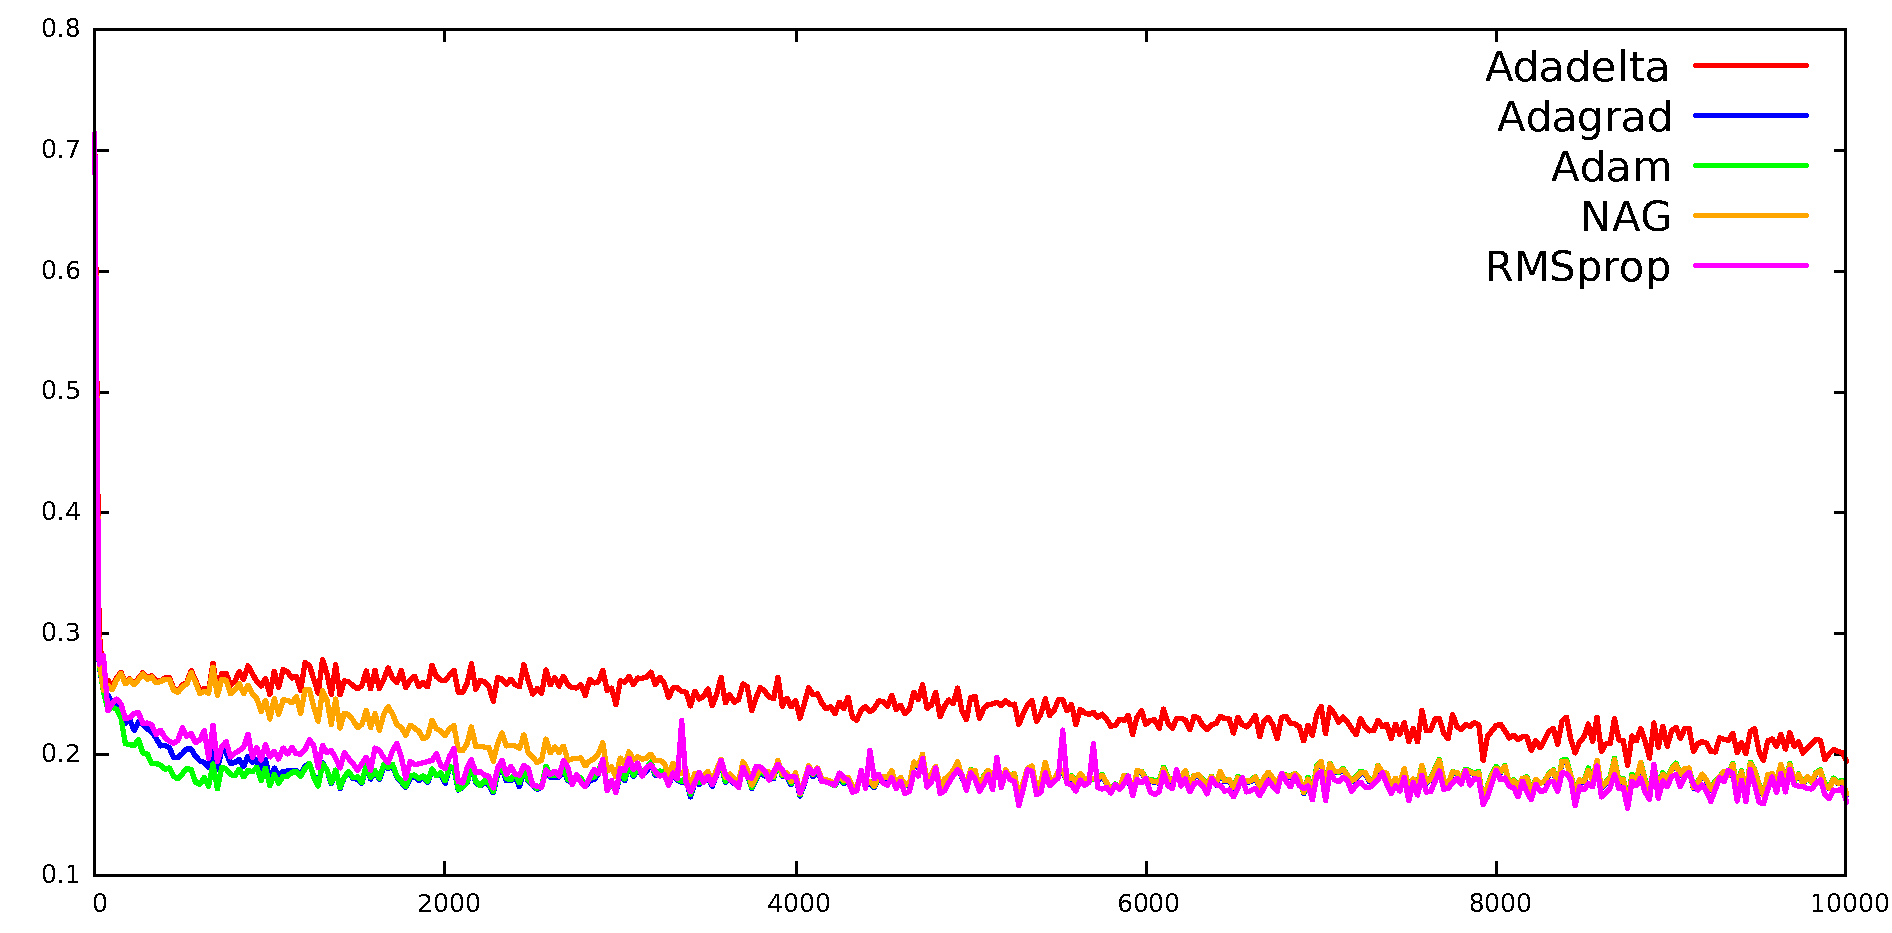
\includegraphics[width=\linewidth]{./images/auto-1.pdf}
\end{figure}
\end{frame}
\begin{frame}{Autoencoder architecture: \texttt{784-1000-500-250-30-30-250-500-1000-10}\footfullcite{hinton} - Training Loss vs Mini-batches} % add citation
\begin{figure}
\centering
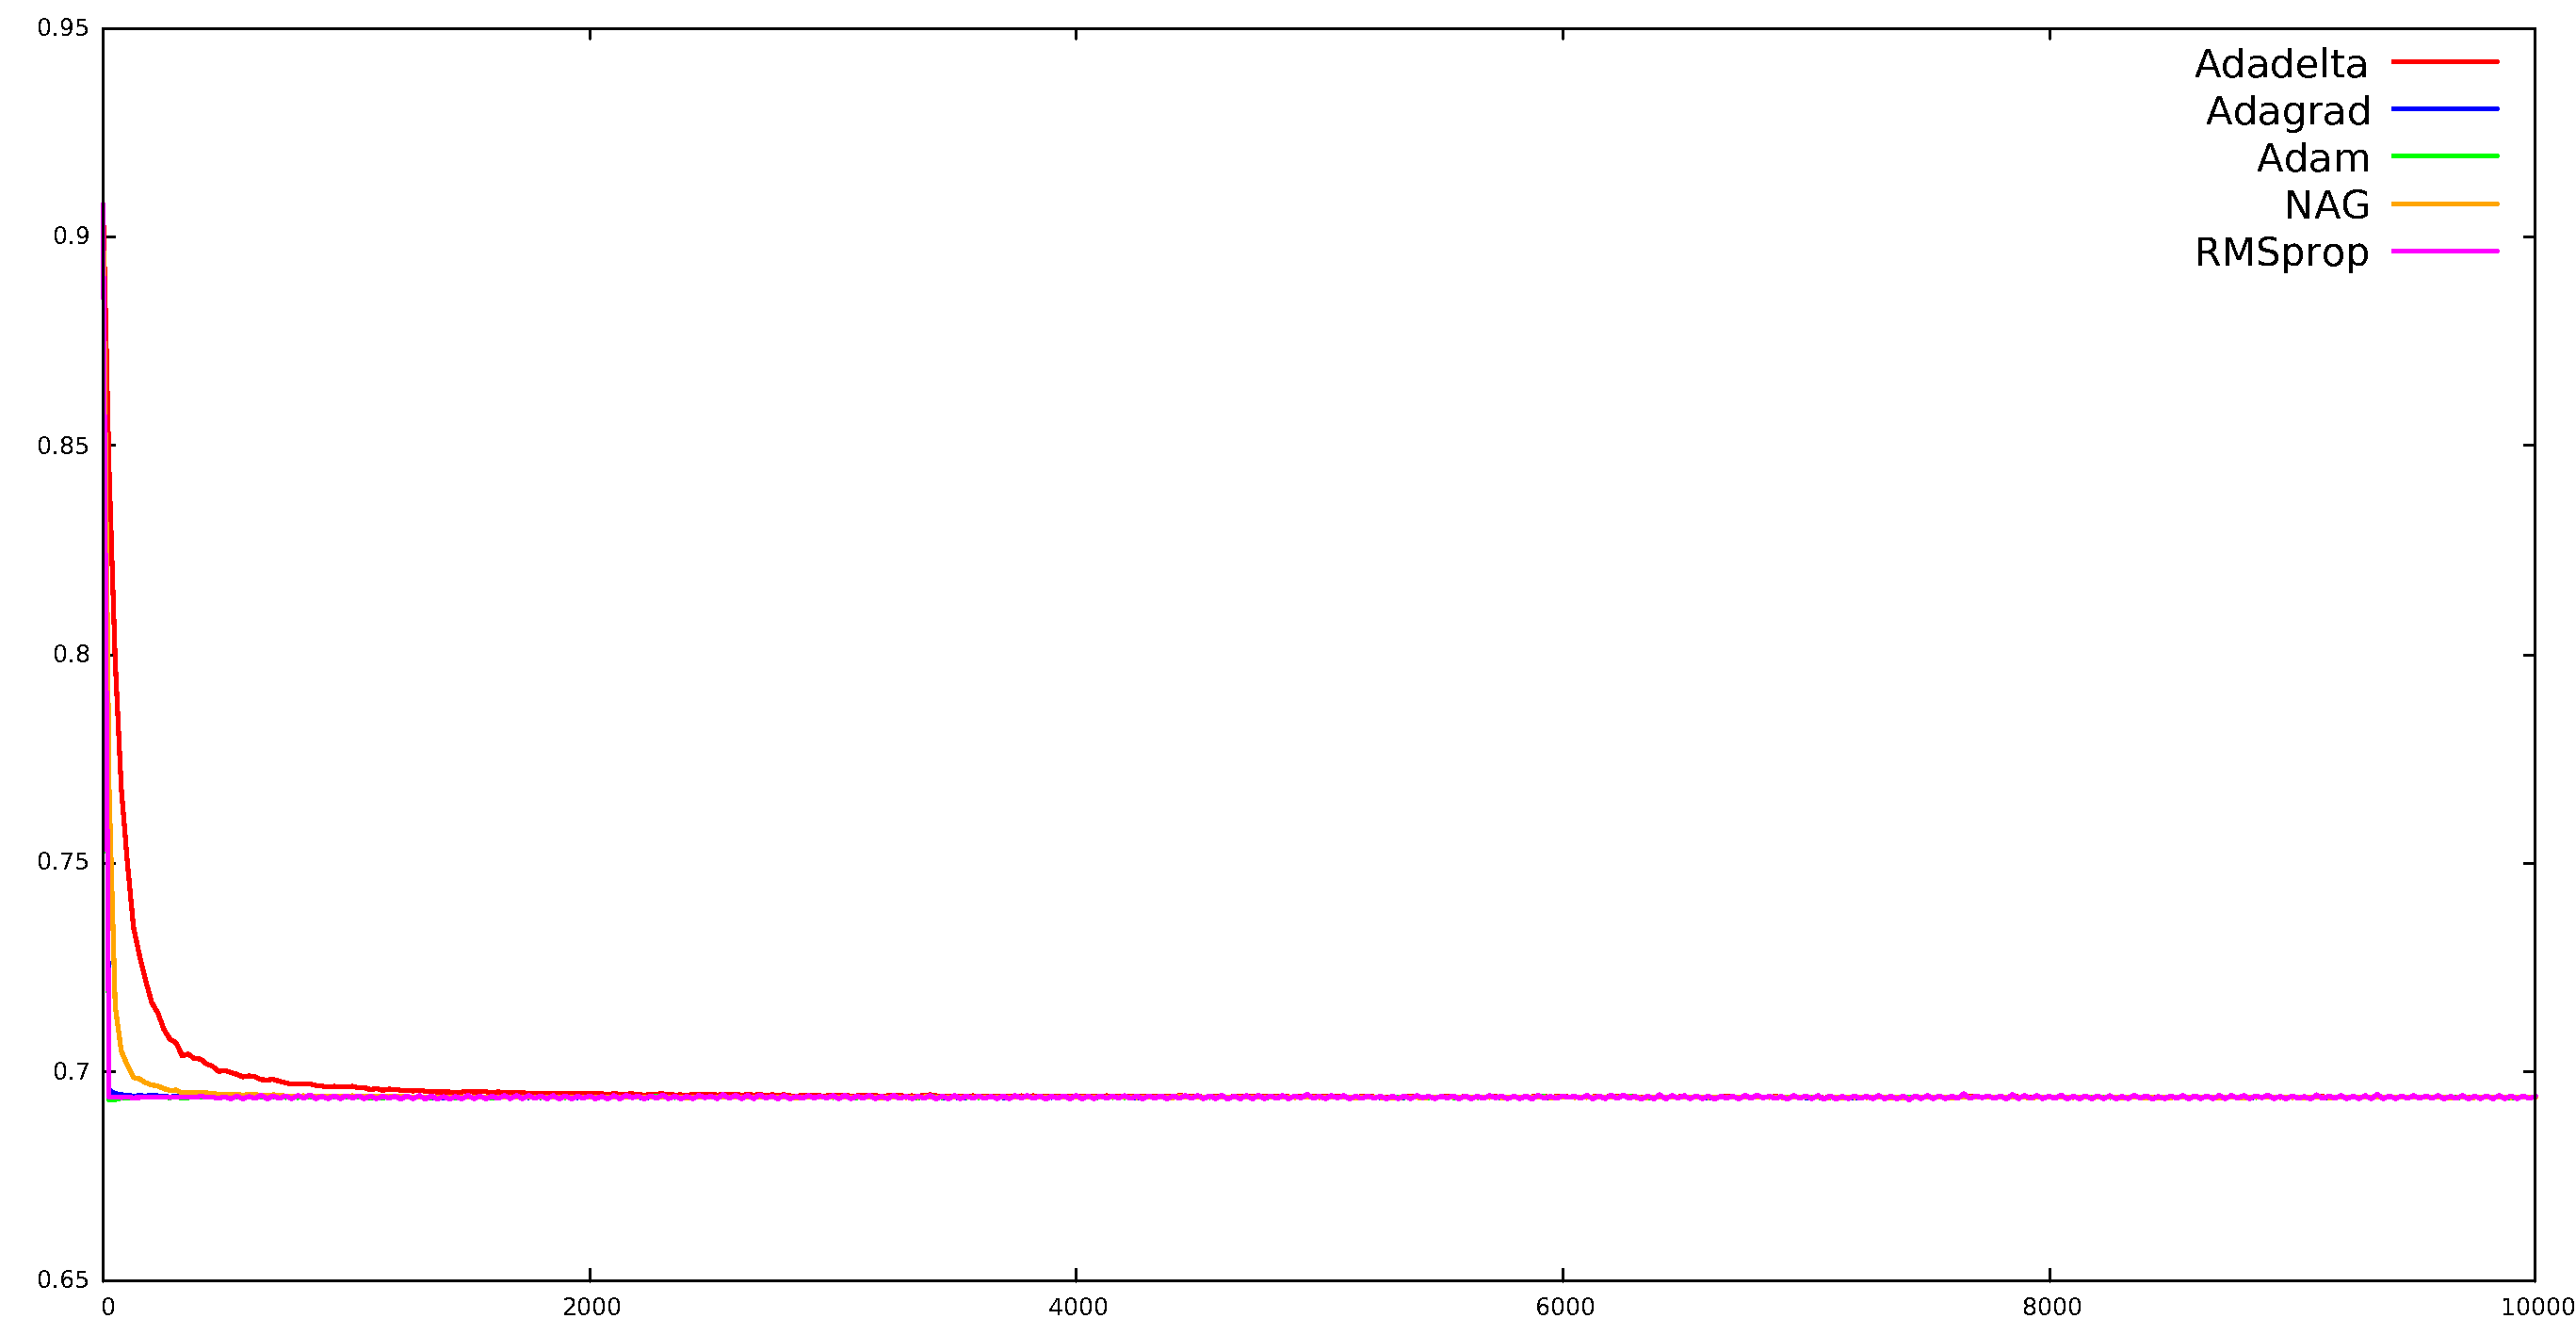
\includegraphics[width=0.9\linewidth]{./images/auto-2.pdf}
\end{figure}
\end{frame}

\subsection{Deep Learning Experiments: GANs}
\begin{frame}{Deep Convolutional Generative Adversarial Networks\footfullcite{dcgan}} %add citation
\begin{itemize}
\item<1->{Used a specialized architecture for generator and discriminator for MNIST digits based on Deep Convolutional GANs}
\item<2->{Run for 50000 iterations, and noted the variations of generator loss and discriminator loss with time for Adam optimizer and Nesterov's Accelerated Gradient}
\end{itemize}
\end{frame}

\begin{frame}{Generator Loss with time}
\begin{figure}
\centering
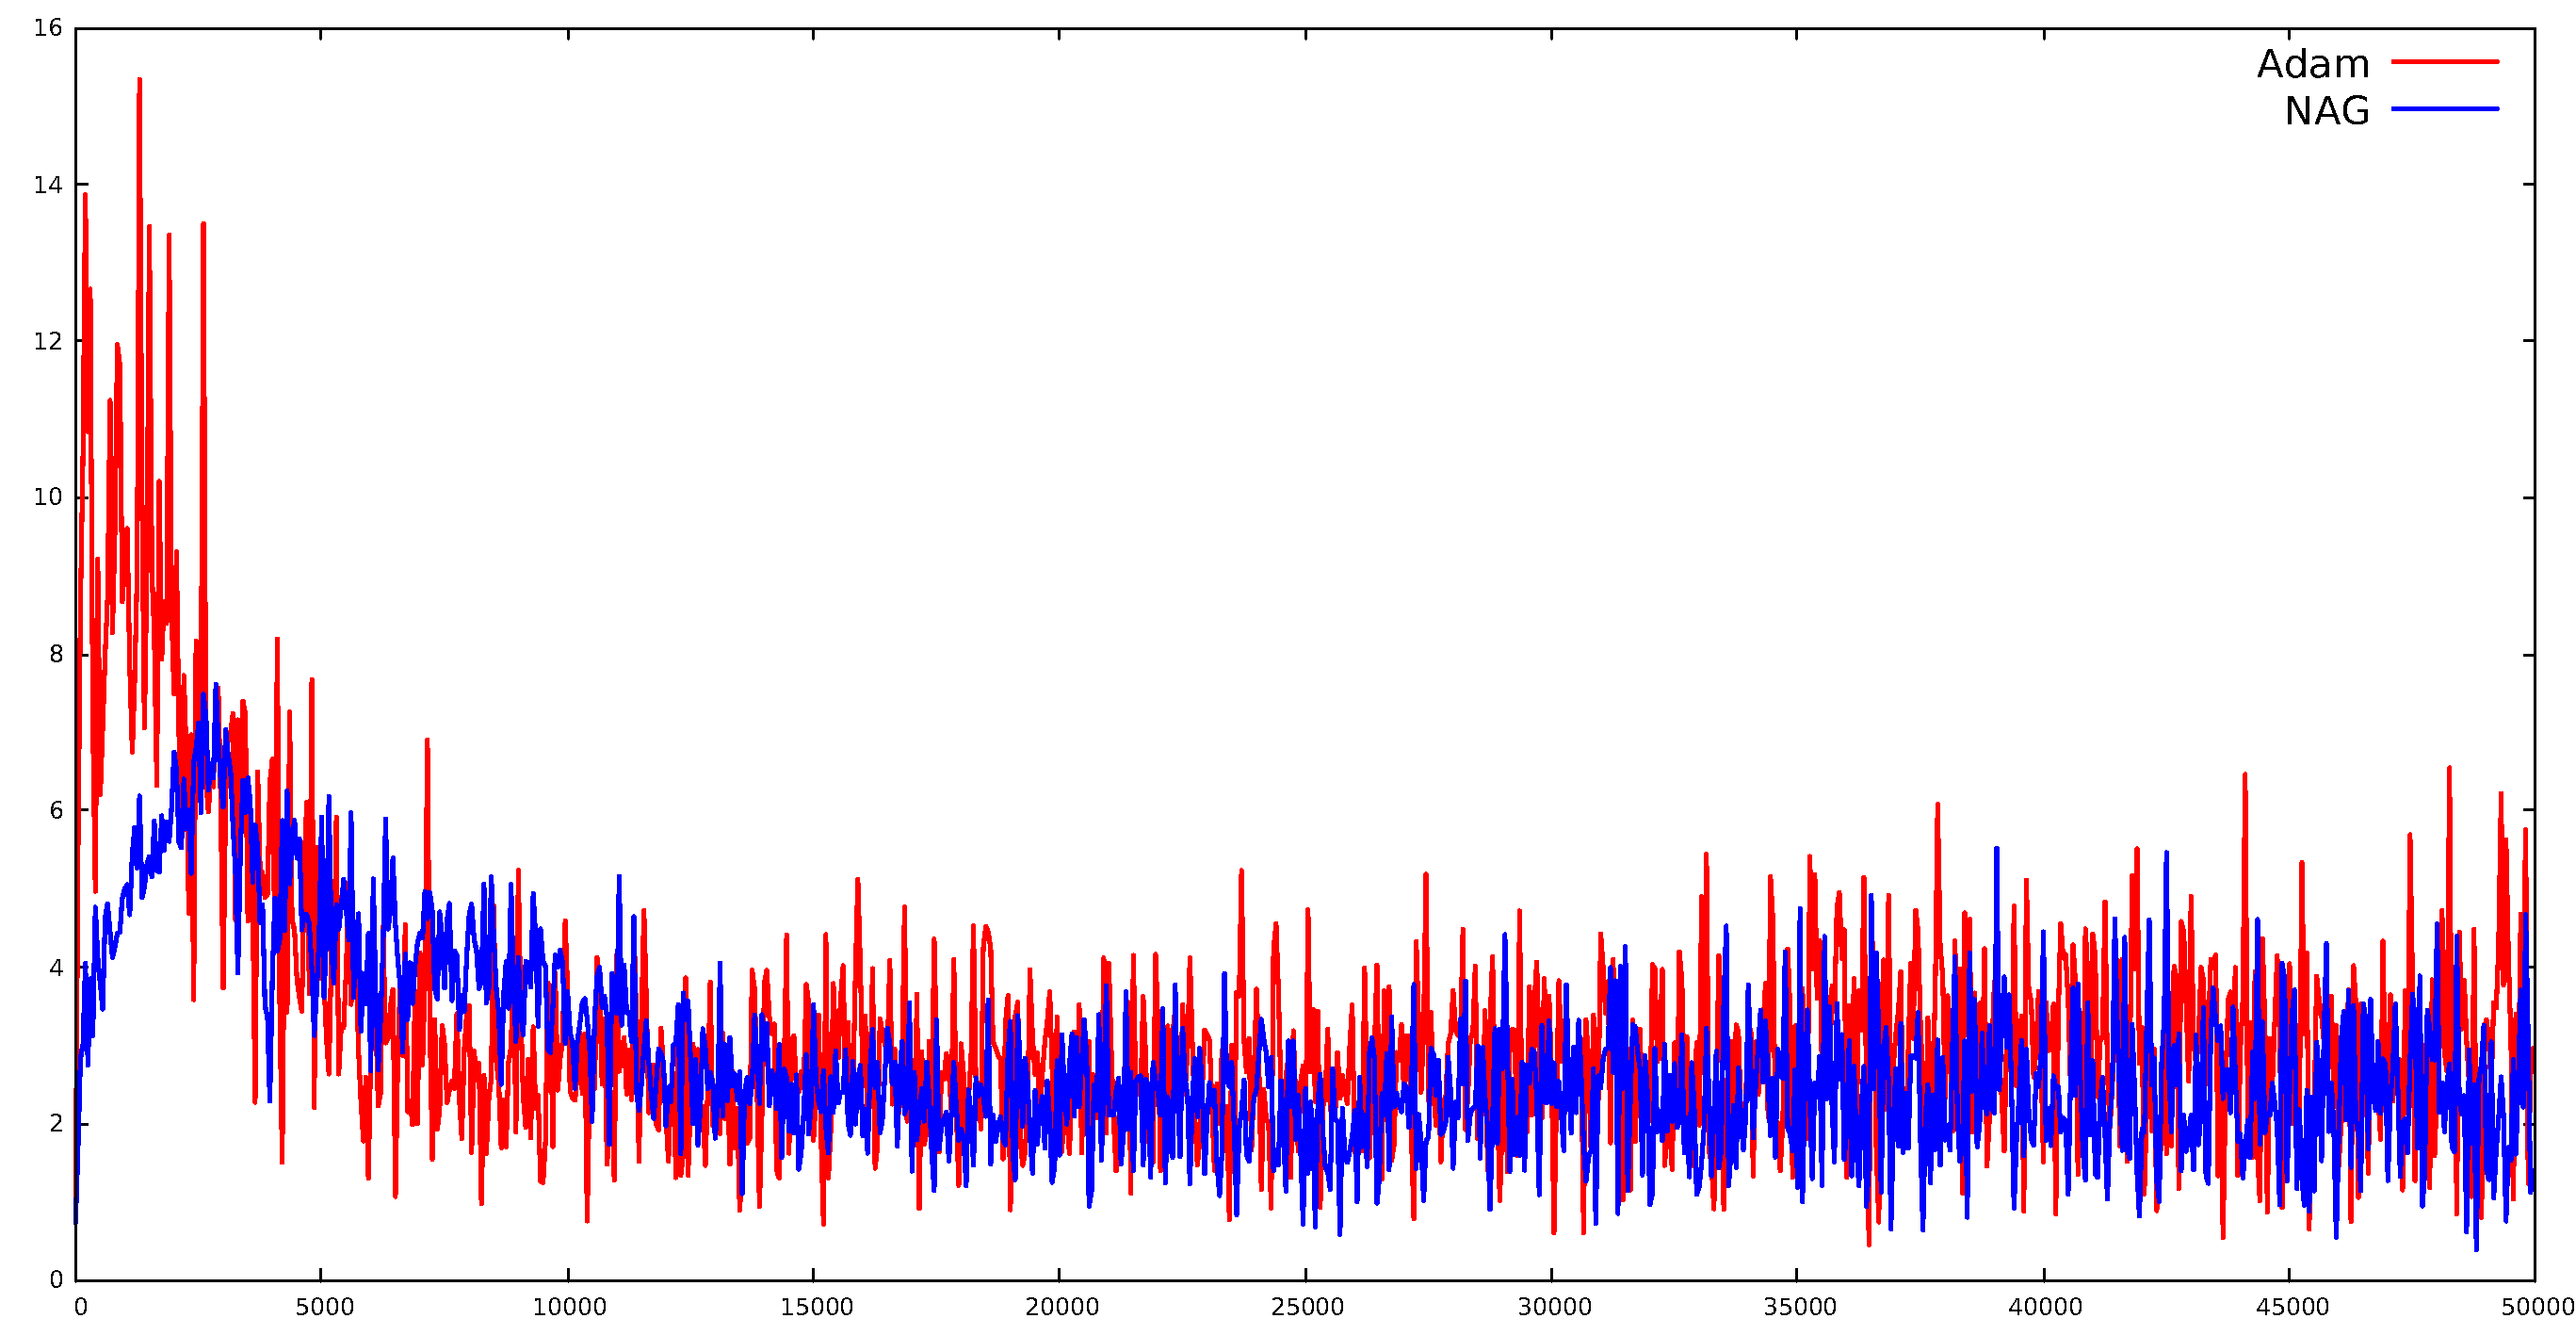
\includegraphics[width=\linewidth]{./images/genr-gan.pdf}
\end{figure}
\end{frame}
\begin{frame}{Discriminator Loss with time}
\begin{figure}
\centering
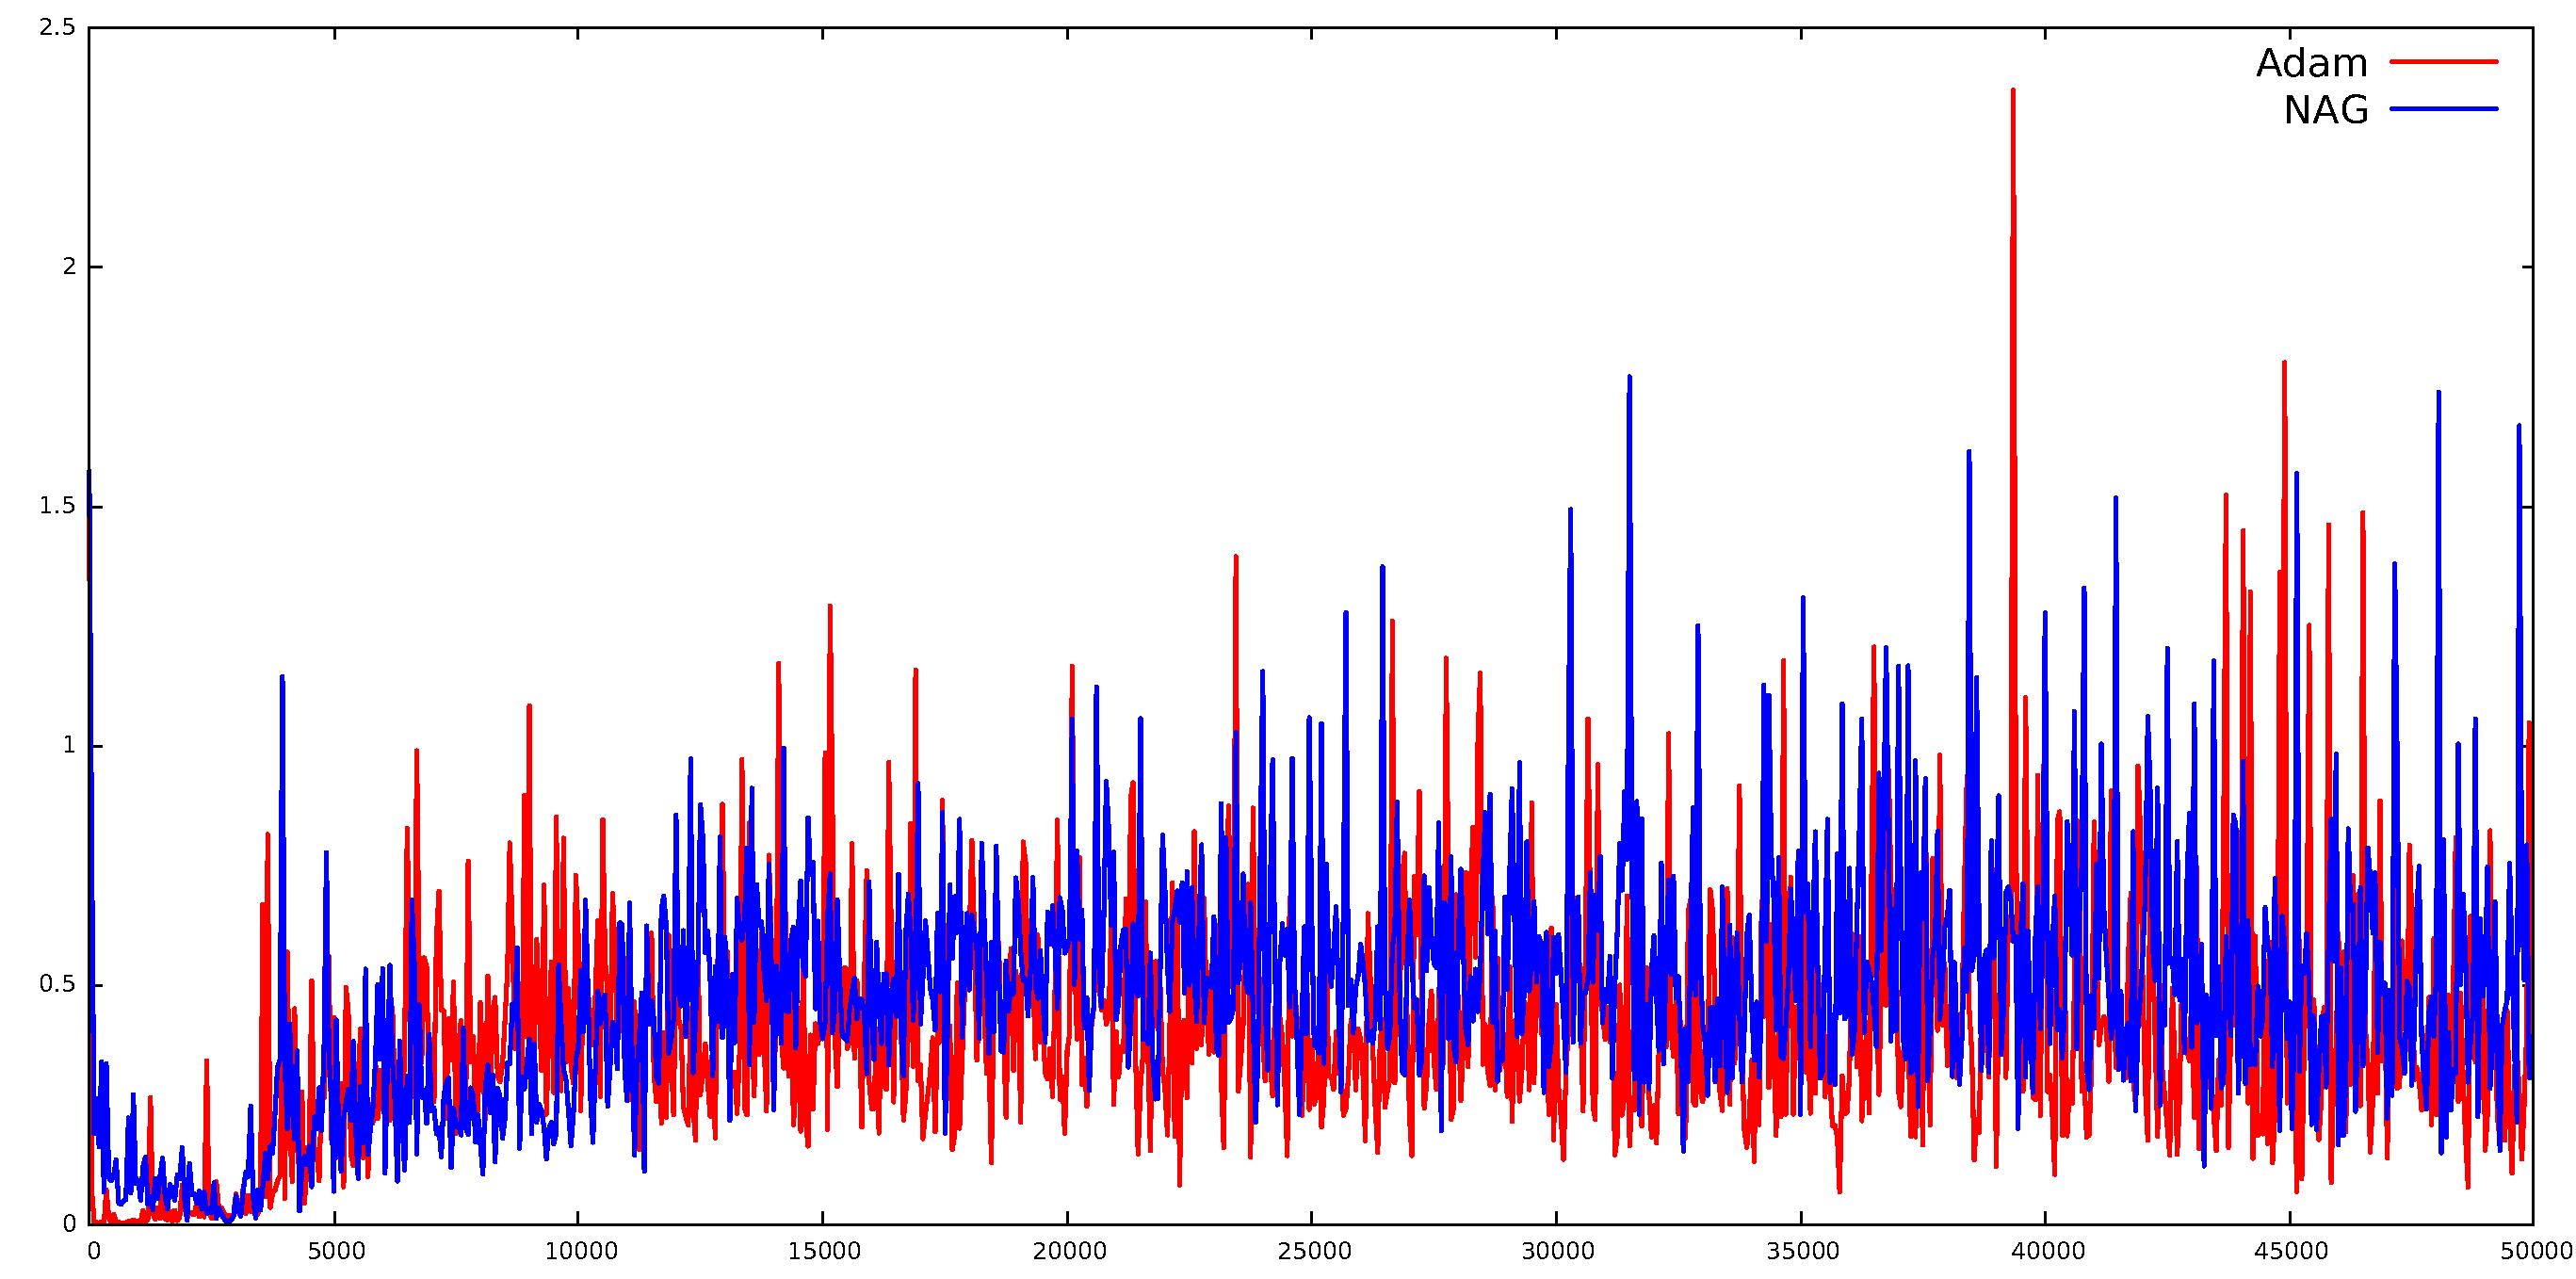
\includegraphics[width=\linewidth]{./images/disc-gan.pdf}
\end{figure}
\end{frame}

\begin{frame}{Quality of Images Generated}
\begin{columns}
\column{0.475\linewidth}
\centering
\textbf{Using ADAM optimizer}
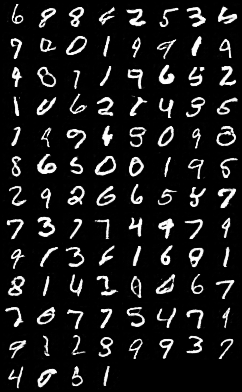
\includegraphics[width=0.75\textwidth]{./images/adam-dcgan.png}
\column{0.475\linewidth}
\centering
\textbf{Using Accelerated Gradient}
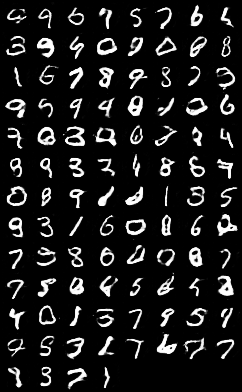
\includegraphics[width=0.75\textwidth]{./images/nag-dcgan.png}
\end{columns}
\end{frame}

\section{Conclusion}
\begin{frame}{Our conclusions from the experiments conducted}
\begin{itemize}
\item<1->{Experiments show that adaptive gradient methods in fact, only have a marginal benefit}
\item<2->{This concurs with the claim put forward by Wilson \textit{et al}\footfullcite{marginaladaptivegradients} about the marginal benefits of Adaptive Gradient Methods}
\item<3->{Hype or Hallelujah? \emph{Hype} it is!!}
\end{itemize}
\end{frame}

\begin{frame}
\Huge{Thank You\footnotetext{Code Available at \url{https://github.com/vishwakftw/CS6230-OML}}}
\end{frame}
\end{document}
